\documentclass[twoside]{book}

% Packages required by doxygen
\usepackage{fixltx2e}
\usepackage{calc}
\usepackage{doxygen}
\usepackage[export]{adjustbox} % also loads graphicx
\usepackage{graphicx}
\usepackage[utf8]{inputenc}
\usepackage{makeidx}
\usepackage{multicol}
\usepackage{multirow}
\PassOptionsToPackage{warn}{textcomp}
\usepackage{textcomp}
\usepackage[nointegrals]{wasysym}
\usepackage[table]{xcolor}

% Font selection
\usepackage[T1]{fontenc}
\usepackage[scaled=.90]{helvet}
\usepackage{courier}
\usepackage{amssymb}
\usepackage{sectsty}
\renewcommand{\familydefault}{\sfdefault}
\allsectionsfont{%
  \fontseries{bc}\selectfont%
  \color{darkgray}%
}
\renewcommand{\DoxyLabelFont}{%
  \fontseries{bc}\selectfont%
  \color{darkgray}%
}
\newcommand{\+}{\discretionary{\mbox{\scriptsize$\hookleftarrow$}}{}{}}

% Page & text layout
\usepackage{geometry}
\geometry{%
  a4paper,%
  top=2.5cm,%
  bottom=2.5cm,%
  left=2.5cm,%
  right=2.5cm%
}
\tolerance=750
\hfuzz=15pt
\hbadness=750
\setlength{\emergencystretch}{15pt}
\setlength{\parindent}{0cm}
\setlength{\parskip}{0.2cm}
\makeatletter
\renewcommand{\paragraph}{%
  \@startsection{paragraph}{4}{0ex}{-1.0ex}{1.0ex}{%
    \normalfont\normalsize\bfseries\SS@parafont%
  }%
}
\renewcommand{\subparagraph}{%
  \@startsection{subparagraph}{5}{0ex}{-1.0ex}{1.0ex}{%
    \normalfont\normalsize\bfseries\SS@subparafont%
  }%
}
\makeatother

% Headers & footers
\usepackage{fancyhdr}
\pagestyle{fancyplain}
\fancyhead[LE]{\fancyplain{}{\bfseries\thepage}}
\fancyhead[CE]{\fancyplain{}{}}
\fancyhead[RE]{\fancyplain{}{\bfseries\leftmark}}
\fancyhead[LO]{\fancyplain{}{\bfseries\rightmark}}
\fancyhead[CO]{\fancyplain{}{}}
\fancyhead[RO]{\fancyplain{}{\bfseries\thepage}}
\fancyfoot[LE]{\fancyplain{}{}}
\fancyfoot[CE]{\fancyplain{}{}}
\fancyfoot[RE]{\fancyplain{}{\bfseries\scriptsize Generated on Mon Jan 5 2015 16\+:55\+:32 for Ci224 by Doxygen }}
\fancyfoot[LO]{\fancyplain{}{\bfseries\scriptsize Generated on Mon Jan 5 2015 16\+:55\+:32 for Ci224 by Doxygen }}
\fancyfoot[CO]{\fancyplain{}{}}
\fancyfoot[RO]{\fancyplain{}{}}
\renewcommand{\footrulewidth}{0.4pt}
\renewcommand{\chaptermark}[1]{%
  \markboth{#1}{}%
}
\renewcommand{\sectionmark}[1]{%
  \markright{\thesection\ #1}%
}

% Indices & bibliography
\usepackage{natbib}
\usepackage[titles]{tocloft}
\setcounter{tocdepth}{3}
\setcounter{secnumdepth}{5}
\makeindex

% Hyperlinks (required, but should be loaded last)
\usepackage{ifpdf}
\ifpdf
  \usepackage[pdftex,pagebackref=true]{hyperref}
\else
  \usepackage[ps2pdf,pagebackref=true]{hyperref}
\fi
\hypersetup{%
  colorlinks=true,%
  linkcolor=blue,%
  citecolor=blue,%
  unicode%
}

% Custom commands
\newcommand{\clearemptydoublepage}{%
  \newpage{\pagestyle{empty}\cleardoublepage}%
}


%===== C O N T E N T S =====

\begin{document}

% Titlepage & ToC
\hypersetup{pageanchor=false,
             bookmarks=true,
             bookmarksnumbered=true,
             pdfencoding=unicode
            }
\pagenumbering{roman}
\begin{titlepage}
\vspace*{7cm}
\begin{center}%
{\Large Ci224 }\\
\vspace*{1cm}
{\large Generated by Doxygen 1.8.9.1}\\
\vspace*{0.5cm}
{\small Mon Jan 5 2015 16:55:32}\\
\end{center}
\end{titlepage}
\clearemptydoublepage
\tableofcontents
\clearemptydoublepage
\pagenumbering{arabic}
\hypersetup{pageanchor=true}

%--- Begin generated contents ---
\chapter{Bug List}
\label{bug}
\hypertarget{bug}{}

\begin{DoxyRefList}
\item[\label{bug__bug000001}%
\hypertarget{bug__bug000001}{}%
Member \hyperlink{class_camera_a6ca725d7a02cc423d220a849140fc0aa}{Camera\+:\+:handle\+Movement} (S\+D\+L\+\_\+\+Event $\ast$e)]movement does not work as intended. camera will move for a certain amount then stop. also camera suffers from gimble lock. need to move over to quaternions in the future.  
\item[\label{bug__bug000002}%
\hypertarget{bug__bug000002}{}%
Member \hyperlink{class_time_a385b4c0869ed969b266535ae835d135d}{Time\+:\+:Delta\+Time} ()]Does not wotk as expected. Wanted a function that would act like Unity3ds Time.\+deltatime 
\end{DoxyRefList}
\chapter{Class Index}
\section{Class List}
Here are the classes, structs, unions and interfaces with brief descriptions\+:\begin{DoxyCompactList}
\item\contentsline{section}{\hyperlink{class_camera}{Camera} }{\pageref{class_camera}}{}
\item\contentsline{section}{\hyperlink{class_game}{Game} }{\pageref{class_game}}{}
\item\contentsline{section}{\hyperlink{classimage_loader}{image\+Loader} }{\pageref{classimage_loader}}{}
\item\contentsline{section}{\hyperlink{class_shader}{Shader} }{\pageref{class_shader}}{}
\item\contentsline{section}{\hyperlink{class_time}{Time} }{\pageref{class_time}}{}
\end{DoxyCompactList}

\chapter{File Index}
\section{File List}
Here is a list of all files with brief descriptions\+:\begin{DoxyCompactList}
\item\contentsline{section}{\hyperlink{_camera_8cpp}{Camera.\+cpp} }{\pageref{_camera_8cpp}}{}
\item\contentsline{section}{\hyperlink{_camera_8h}{Camera.\+h} }{\pageref{_camera_8h}}{}
\item\contentsline{section}{\hyperlink{game_8cpp}{game.\+cpp} }{\pageref{game_8cpp}}{}
\item\contentsline{section}{\hyperlink{game_8h}{game.\+h} }{\pageref{game_8h}}{}
\item\contentsline{section}{\hyperlink{image_loader_8cpp}{image\+Loader.\+cpp} }{\pageref{image_loader_8cpp}}{}
\item\contentsline{section}{\hyperlink{image_loader_8h}{image\+Loader.\+h} }{\pageref{image_loader_8h}}{}
\item\contentsline{section}{\hyperlink{main_8cpp}{main.\+cpp} }{\pageref{main_8cpp}}{}
\item\contentsline{section}{\hyperlink{shader_8cpp}{shader.\+cpp} }{\pageref{shader_8cpp}}{}
\item\contentsline{section}{\hyperlink{shader_8h}{shader.\+h} }{\pageref{shader_8h}}{}
\item\contentsline{section}{\hyperlink{_time_8cpp}{Time.\+cpp} }{\pageref{_time_8cpp}}{}
\item\contentsline{section}{\hyperlink{_time_8h}{Time.\+h} }{\pageref{_time_8h}}{}
\item\contentsline{section}{build/\+C\+Make\+Files/2.\+8.\+12.\+2/\+Compiler\+Id\+C/\hyperlink{_c_make_c_compiler_id_8c}{C\+Make\+C\+Compiler\+Id.\+c} }{\pageref{_c_make_c_compiler_id_8c}}{}
\item\contentsline{section}{build/\+C\+Make\+Files/2.\+8.\+12.\+2/\+Compiler\+Id\+C\+X\+X/\hyperlink{_c_make_c_x_x_compiler_id_8cpp}{C\+Make\+C\+X\+X\+Compiler\+Id.\+cpp} }{\pageref{_c_make_c_x_x_compiler_id_8cpp}}{}
\end{DoxyCompactList}

\chapter{Class Documentation}
\hypertarget{class_camera}{}\section{Camera Class Reference}
\label{class_camera}\index{Camera@{Camera}}


{\ttfamily \#include $<$Camera.\+h$>$}



Collaboration diagram for Camera\+:\nopagebreak
\begin{figure}[H]
\begin{center}
\leavevmode
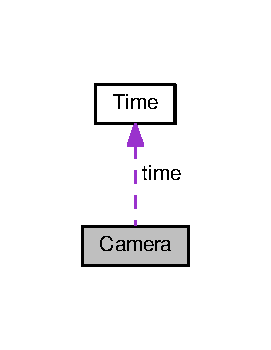
\includegraphics[width=130pt]{class_camera__coll__graph}
\end{center}
\end{figure}
\subsection*{Public Member Functions}
\begin{DoxyCompactItemize}
\item 
\hyperlink{class_camera_a01f94c3543f56ede7af49dc778f19331}{Camera} ()
\item 
void \hyperlink{class_camera_a6ca725d7a02cc423d220a849140fc0aa}{handle\+Movement} (S\+D\+L\+\_\+\+Event $\ast$e)
\item 
void \hyperlink{class_camera_a42cda7239981a5618660d04bd5893556}{update} ()
\end{DoxyCompactItemize}
\subsection*{Public Attributes}
\begin{DoxyCompactItemize}
\item 
glm\+::vec3 \hyperlink{class_camera_a424bcf971a87506ba6770f2c5c1073f0}{camera\+Pos}
\item 
glm\+::vec3 \hyperlink{class_camera_ad641b25d477900ac4f3cd859ac14e8f7}{camera\+Dir} = glm\+::vec3(0.\+0f, 0.\+0f, -\/1.\+0f)
\item 
glm\+::vec3 \hyperlink{class_camera_a517042b127746997f9472d51bbae2610}{camera\+Up} = glm\+::vec3(0.\+0f, 1.\+0f, 0.\+0f)
\item 
int \hyperlink{class_camera_a76f82934e9d29f80a6067b900d750b55}{x\+Pos}
\item 
int \hyperlink{class_camera_ae73c8dc0602e7849e7ec730f9acc1954}{y\+Pos}
\item 
G\+Lfloat \hyperlink{class_camera_a0c41085cad802bae1026706d23688034}{x\+Off\+Set}
\item 
G\+Lfloat \hyperlink{class_camera_a6d394f402515409bac177801ab11619b}{y\+Off\+Set}
\item 
G\+Lfloat \hyperlink{class_camera_a8f67cd3183810d8d675d38cc62af966a}{camera\+Speed} = 1.\+0f
\item 
glm\+::mat4 \hyperlink{class_camera_add93fedd6b9a6a6e2c784aeda624de83}{view}
\item 
glm\+::mat4 \hyperlink{class_camera_a43555a0ae83f9ec696ee257e5fd48cf2}{projection}
\item 
\hyperlink{class_time}{Time} $\ast$ \hyperlink{class_camera_a5944842935bf511fb1720f50f0f426da}{time}
\end{DoxyCompactItemize}


\subsection{Detailed Description}


Definition at line 18 of file Camera.\+h.



\subsection{Constructor \& Destructor Documentation}
\hypertarget{class_camera_a01f94c3543f56ede7af49dc778f19331}{}\index{Camera@{Camera}!Camera@{Camera}}
\index{Camera@{Camera}!Camera@{Camera}}
\subsubsection[{Camera}]{\setlength{\rightskip}{0pt plus 5cm}Camera\+::\+Camera (
\begin{DoxyParamCaption}
{}
\end{DoxyParamCaption}
)}\label{class_camera_a01f94c3543f56ede7af49dc778f19331}
Initialise Variables; 

Definition at line 7 of file Camera.\+cpp.



\subsection{Member Function Documentation}
\hypertarget{class_camera_a6ca725d7a02cc423d220a849140fc0aa}{}\index{Camera@{Camera}!handle\+Movement@{handle\+Movement}}
\index{handle\+Movement@{handle\+Movement}!Camera@{Camera}}
\subsubsection[{handle\+Movement}]{\setlength{\rightskip}{0pt plus 5cm}void Camera\+::handle\+Movement (
\begin{DoxyParamCaption}
\item[{S\+D\+L\+\_\+\+Event $\ast$}]{e}
\end{DoxyParamCaption}
)}\label{class_camera_a6ca725d7a02cc423d220a849140fc0aa}
Handle input form passed in main\+Event struct. \begin{DoxyRefDesc}{Bug}
\item[\hyperlink{bug__bug000001}{Bug}]movement does not work as intended. camera will move for a certain amount then stop. also camera suffers from gimble lock. need to move over to quaternions in the future. \end{DoxyRefDesc}
used for debug

Definition at line 24 of file Camera.\+cpp.



Here is the caller graph for this function\+:\nopagebreak
\begin{figure}[H]
\begin{center}
\leavevmode
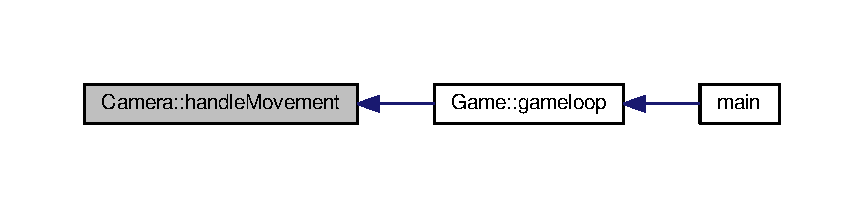
\includegraphics[width=350pt]{class_camera_a6ca725d7a02cc423d220a849140fc0aa_icgraph}
\end{center}
\end{figure}


\hypertarget{class_camera_a42cda7239981a5618660d04bd5893556}{}\index{Camera@{Camera}!update@{update}}
\index{update@{update}!Camera@{Camera}}
\subsubsection[{update}]{\setlength{\rightskip}{0pt plus 5cm}void Camera\+::update (
\begin{DoxyParamCaption}
{}
\end{DoxyParamCaption}
)}\label{class_camera_a42cda7239981a5618660d04bd5893556}


Definition at line 89 of file Camera.\+cpp.



Here is the caller graph for this function\+:\nopagebreak
\begin{figure}[H]
\begin{center}
\leavevmode
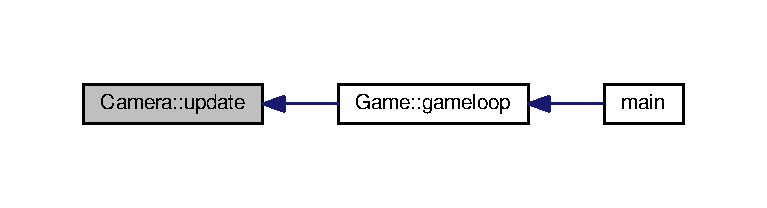
\includegraphics[width=350pt]{class_camera_a42cda7239981a5618660d04bd5893556_icgraph}
\end{center}
\end{figure}




\subsection{Member Data Documentation}
\hypertarget{class_camera_ad641b25d477900ac4f3cd859ac14e8f7}{}\index{Camera@{Camera}!camera\+Dir@{camera\+Dir}}
\index{camera\+Dir@{camera\+Dir}!Camera@{Camera}}
\subsubsection[{camera\+Dir}]{\setlength{\rightskip}{0pt plus 5cm}glm\+::vec3 Camera\+::camera\+Dir = glm\+::vec3(0.\+0f, 0.\+0f, -\/1.\+0f)}\label{class_camera_ad641b25d477900ac4f3cd859ac14e8f7}


Definition at line 24 of file Camera.\+h.

\hypertarget{class_camera_a424bcf971a87506ba6770f2c5c1073f0}{}\index{Camera@{Camera}!camera\+Pos@{camera\+Pos}}
\index{camera\+Pos@{camera\+Pos}!Camera@{Camera}}
\subsubsection[{camera\+Pos}]{\setlength{\rightskip}{0pt plus 5cm}glm\+::vec3 Camera\+::camera\+Pos}\label{class_camera_a424bcf971a87506ba6770f2c5c1073f0}


Definition at line 23 of file Camera.\+h.

\hypertarget{class_camera_a8f67cd3183810d8d675d38cc62af966a}{}\index{Camera@{Camera}!camera\+Speed@{camera\+Speed}}
\index{camera\+Speed@{camera\+Speed}!Camera@{Camera}}
\subsubsection[{camera\+Speed}]{\setlength{\rightskip}{0pt plus 5cm}G\+Lfloat Camera\+::camera\+Speed = 1.\+0f}\label{class_camera_a8f67cd3183810d8d675d38cc62af966a}


Definition at line 30 of file Camera.\+h.

\hypertarget{class_camera_a517042b127746997f9472d51bbae2610}{}\index{Camera@{Camera}!camera\+Up@{camera\+Up}}
\index{camera\+Up@{camera\+Up}!Camera@{Camera}}
\subsubsection[{camera\+Up}]{\setlength{\rightskip}{0pt plus 5cm}glm\+::vec3 Camera\+::camera\+Up = glm\+::vec3(0.\+0f, 1.\+0f, 0.\+0f)}\label{class_camera_a517042b127746997f9472d51bbae2610}


Definition at line 25 of file Camera.\+h.

\hypertarget{class_camera_a43555a0ae83f9ec696ee257e5fd48cf2}{}\index{Camera@{Camera}!projection@{projection}}
\index{projection@{projection}!Camera@{Camera}}
\subsubsection[{projection}]{\setlength{\rightskip}{0pt plus 5cm}glm\+::mat4 Camera\+::projection}\label{class_camera_a43555a0ae83f9ec696ee257e5fd48cf2}


Definition at line 36 of file Camera.\+h.

\hypertarget{class_camera_a5944842935bf511fb1720f50f0f426da}{}\index{Camera@{Camera}!time@{time}}
\index{time@{time}!Camera@{Camera}}
\subsubsection[{time}]{\setlength{\rightskip}{0pt plus 5cm}{\bf Time}$\ast$ Camera\+::time}\label{class_camera_a5944842935bf511fb1720f50f0f426da}


Definition at line 37 of file Camera.\+h.

\hypertarget{class_camera_add93fedd6b9a6a6e2c784aeda624de83}{}\index{Camera@{Camera}!view@{view}}
\index{view@{view}!Camera@{Camera}}
\subsubsection[{view}]{\setlength{\rightskip}{0pt plus 5cm}glm\+::mat4 Camera\+::view}\label{class_camera_add93fedd6b9a6a6e2c784aeda624de83}


Definition at line 35 of file Camera.\+h.

\hypertarget{class_camera_a0c41085cad802bae1026706d23688034}{}\index{Camera@{Camera}!x\+Off\+Set@{x\+Off\+Set}}
\index{x\+Off\+Set@{x\+Off\+Set}!Camera@{Camera}}
\subsubsection[{x\+Off\+Set}]{\setlength{\rightskip}{0pt plus 5cm}G\+Lfloat Camera\+::x\+Off\+Set}\label{class_camera_a0c41085cad802bae1026706d23688034}


Definition at line 29 of file Camera.\+h.

\hypertarget{class_camera_a76f82934e9d29f80a6067b900d750b55}{}\index{Camera@{Camera}!x\+Pos@{x\+Pos}}
\index{x\+Pos@{x\+Pos}!Camera@{Camera}}
\subsubsection[{x\+Pos}]{\setlength{\rightskip}{0pt plus 5cm}int Camera\+::x\+Pos}\label{class_camera_a76f82934e9d29f80a6067b900d750b55}


Definition at line 27 of file Camera.\+h.

\hypertarget{class_camera_a6d394f402515409bac177801ab11619b}{}\index{Camera@{Camera}!y\+Off\+Set@{y\+Off\+Set}}
\index{y\+Off\+Set@{y\+Off\+Set}!Camera@{Camera}}
\subsubsection[{y\+Off\+Set}]{\setlength{\rightskip}{0pt plus 5cm}G\+Lfloat Camera\+::y\+Off\+Set}\label{class_camera_a6d394f402515409bac177801ab11619b}


Definition at line 29 of file Camera.\+h.

\hypertarget{class_camera_ae73c8dc0602e7849e7ec730f9acc1954}{}\index{Camera@{Camera}!y\+Pos@{y\+Pos}}
\index{y\+Pos@{y\+Pos}!Camera@{Camera}}
\subsubsection[{y\+Pos}]{\setlength{\rightskip}{0pt plus 5cm}int Camera\+::y\+Pos}\label{class_camera_ae73c8dc0602e7849e7ec730f9acc1954}


Definition at line 28 of file Camera.\+h.



The documentation for this class was generated from the following files\+:\begin{DoxyCompactItemize}
\item 
\hyperlink{_camera_8h}{Camera.\+h}\item 
\hyperlink{_camera_8cpp}{Camera.\+cpp}\end{DoxyCompactItemize}

\hypertarget{class_game}{}\section{Game Class Reference}
\label{class_game}\index{Game@{Game}}


{\ttfamily \#include $<$game.\+h$>$}

\subsection*{Public Member Functions}
\begin{DoxyCompactItemize}
\item 
\hyperlink{class_game_ad59df6562a58a614fda24622d3715b65}{Game} ()
\item 
\hyperlink{class_game_ae3d112ca6e0e55150d2fdbc704474530}{$\sim$\+Game} ()
\item 
void \hyperlink{class_game_a6f3a33940524b6ba9d83f627ccb14bbf}{init} ()
\item 
void \hyperlink{class_game_a961f632fbe7f4ba08d23fe9edc7711be}{cleanup} ()
\item 
void \hyperlink{class_game_aeae97cec35573c668d3f222a58f53255}{gameloop} ()
\item 
void \hyperlink{class_game_a15ddd769261d923827a3cdf41499c843}{render} ()
\item 
void \hyperlink{class_game_af432b82a96963dd1ad8214625f3a4438}{setup\+Shaders} ()
\item 
void \hyperlink{class_game_ab5ae2734e96b7913dd131208065b4b5a}{load\+Cube} ()
\end{DoxyCompactItemize}


\subsection{Detailed Description}


Definition at line 26 of file game.\+h.



\subsection{Constructor \& Destructor Documentation}
\hypertarget{class_game_ad59df6562a58a614fda24622d3715b65}{}\index{Game@{Game}!Game@{Game}}
\index{Game@{Game}!Game@{Game}}
\subsubsection[{Game}]{\setlength{\rightskip}{0pt plus 5cm}Game\+::\+Game (
\begin{DoxyParamCaption}
{}
\end{DoxyParamCaption}
)}\label{class_game_ad59df6562a58a614fda24622d3715b65}
Initialise variables and create needed objects 

Definition at line 7 of file game.\+cpp.

\hypertarget{class_game_ae3d112ca6e0e55150d2fdbc704474530}{}\index{Game@{Game}!````~Game@{$\sim$\+Game}}
\index{````~Game@{$\sim$\+Game}!Game@{Game}}
\subsubsection[{$\sim$\+Game}]{\setlength{\rightskip}{0pt plus 5cm}Game\+::$\sim$\+Game (
\begin{DoxyParamCaption}
{}
\end{DoxyParamCaption}
)}\label{class_game_ae3d112ca6e0e55150d2fdbc704474530}


Definition at line 15 of file game.\+cpp.



\subsection{Member Function Documentation}
\hypertarget{class_game_a961f632fbe7f4ba08d23fe9edc7711be}{}\index{Game@{Game}!cleanup@{cleanup}}
\index{cleanup@{cleanup}!Game@{Game}}
\subsubsection[{cleanup}]{\setlength{\rightskip}{0pt plus 5cm}void Game\+::cleanup (
\begin{DoxyParamCaption}
{}
\end{DoxyParamCaption}
)}\label{class_game_a961f632fbe7f4ba08d23fe9edc7711be}
Delete open\+G\+L context and cleanup S\+D\+L 

Definition at line 65 of file game.\+cpp.



Here is the caller graph for this function\+:\nopagebreak
\begin{figure}[H]
\begin{center}
\leavevmode
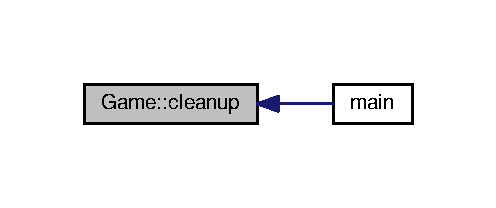
\includegraphics[width=238pt]{class_game_a961f632fbe7f4ba08d23fe9edc7711be_icgraph}
\end{center}
\end{figure}


\hypertarget{class_game_aeae97cec35573c668d3f222a58f53255}{}\index{Game@{Game}!gameloop@{gameloop}}
\index{gameloop@{gameloop}!Game@{Game}}
\subsubsection[{gameloop}]{\setlength{\rightskip}{0pt plus 5cm}void Game\+::gameloop (
\begin{DoxyParamCaption}
{}
\end{DoxyParamCaption}
)}\label{class_game_aeae97cec35573c668d3f222a58f53255}
Main game loop 

Definition at line 75 of file game.\+cpp.



Here is the call graph for this function\+:\nopagebreak
\begin{figure}[H]
\begin{center}
\leavevmode
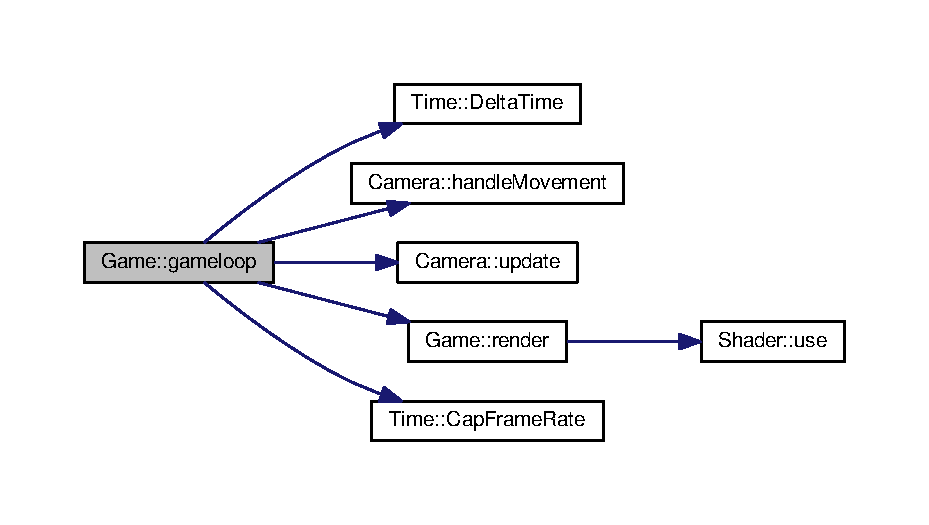
\includegraphics[width=350pt]{class_game_aeae97cec35573c668d3f222a58f53255_cgraph}
\end{center}
\end{figure}




Here is the caller graph for this function\+:\nopagebreak
\begin{figure}[H]
\begin{center}
\leavevmode
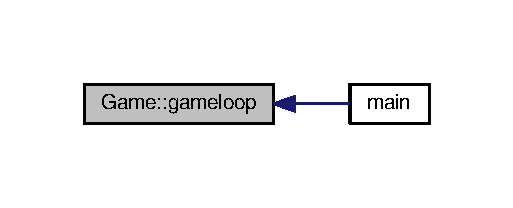
\includegraphics[width=246pt]{class_game_aeae97cec35573c668d3f222a58f53255_icgraph}
\end{center}
\end{figure}


\hypertarget{class_game_a6f3a33940524b6ba9d83f627ccb14bbf}{}\index{Game@{Game}!init@{init}}
\index{init@{init}!Game@{Game}}
\subsubsection[{init}]{\setlength{\rightskip}{0pt plus 5cm}void Game\+::init (
\begin{DoxyParamCaption}
{}
\end{DoxyParamCaption}
)}\label{class_game_a6f3a33940524b6ba9d83f627ccb14bbf}
Intialise S\+D\+L and create open\+G\+L context. load, compile and linking of shaders. Image loading also done. 

Definition at line 25 of file game.\+cpp.



Here is the call graph for this function\+:\nopagebreak
\begin{figure}[H]
\begin{center}
\leavevmode
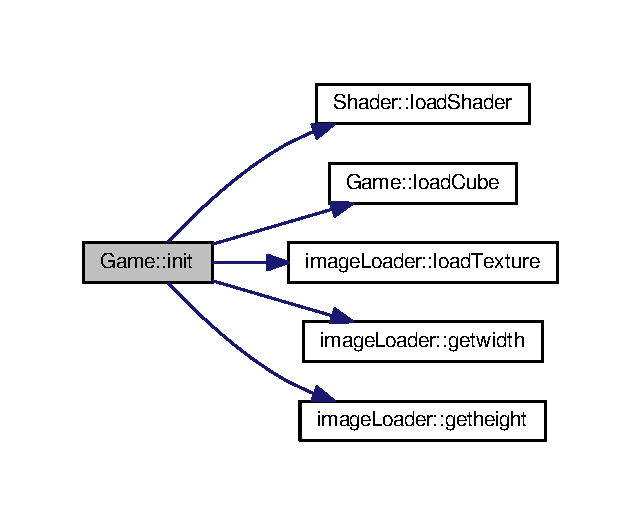
\includegraphics[width=308pt]{class_game_a6f3a33940524b6ba9d83f627ccb14bbf_cgraph}
\end{center}
\end{figure}




Here is the caller graph for this function\+:\nopagebreak
\begin{figure}[H]
\begin{center}
\leavevmode
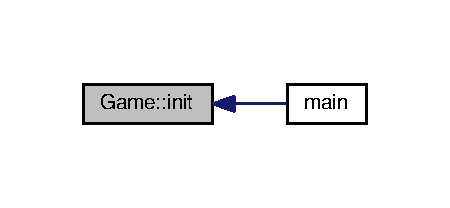
\includegraphics[width=216pt]{class_game_a6f3a33940524b6ba9d83f627ccb14bbf_icgraph}
\end{center}
\end{figure}


\hypertarget{class_game_ab5ae2734e96b7913dd131208065b4b5a}{}\index{Game@{Game}!load\+Cube@{load\+Cube}}
\index{load\+Cube@{load\+Cube}!Game@{Game}}
\subsubsection[{load\+Cube}]{\setlength{\rightskip}{0pt plus 5cm}void Game\+::load\+Cube (
\begin{DoxyParamCaption}
{}
\end{DoxyParamCaption}
)}\label{class_game_ab5ae2734e96b7913dd131208065b4b5a}
Function to load and pass vertices to the Gpu 

Definition at line 192 of file game.\+cpp.



Here is the caller graph for this function\+:\nopagebreak
\begin{figure}[H]
\begin{center}
\leavevmode
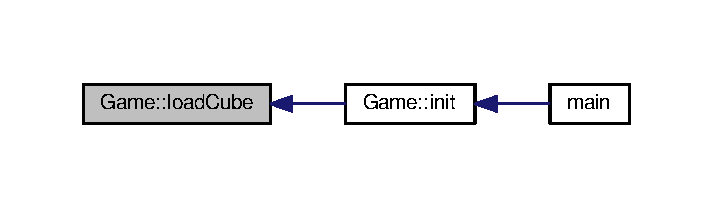
\includegraphics[width=342pt]{class_game_ab5ae2734e96b7913dd131208065b4b5a_icgraph}
\end{center}
\end{figure}


\hypertarget{class_game_a15ddd769261d923827a3cdf41499c843}{}\index{Game@{Game}!render@{render}}
\index{render@{render}!Game@{Game}}
\subsubsection[{render}]{\setlength{\rightskip}{0pt plus 5cm}void Game\+::render (
\begin{DoxyParamCaption}
{}
\end{DoxyParamCaption}
)}\label{class_game_a15ddd769261d923827a3cdf41499c843}
Render function all drawing code currently in here create and fill two 3 dimensional arrays.

Loop through both arrays and render.

Definition at line 108 of file game.\+cpp.



Here is the call graph for this function\+:\nopagebreak
\begin{figure}[H]
\begin{center}
\leavevmode
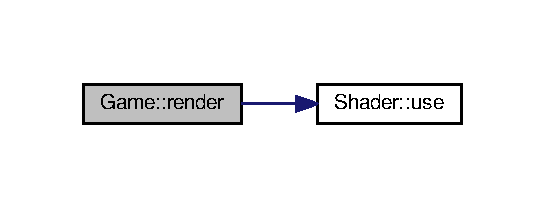
\includegraphics[width=262pt]{class_game_a15ddd769261d923827a3cdf41499c843_cgraph}
\end{center}
\end{figure}




Here is the caller graph for this function\+:\nopagebreak
\begin{figure}[H]
\begin{center}
\leavevmode
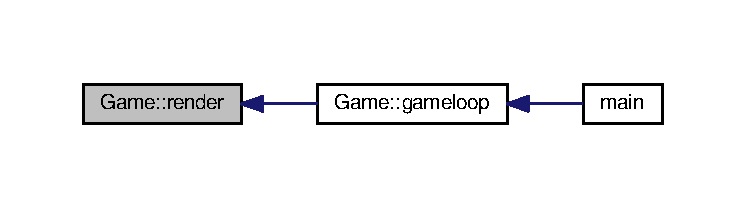
\includegraphics[width=350pt]{class_game_a15ddd769261d923827a3cdf41499c843_icgraph}
\end{center}
\end{figure}


\hypertarget{class_game_af432b82a96963dd1ad8214625f3a4438}{}\index{Game@{Game}!setup\+Shaders@{setup\+Shaders}}
\index{setup\+Shaders@{setup\+Shaders}!Game@{Game}}
\subsubsection[{setup\+Shaders}]{\setlength{\rightskip}{0pt plus 5cm}void Game\+::setup\+Shaders (
\begin{DoxyParamCaption}
{}
\end{DoxyParamCaption}
)}\label{class_game_af432b82a96963dd1ad8214625f3a4438}


The documentation for this class was generated from the following files\+:\begin{DoxyCompactItemize}
\item 
\hyperlink{game_8h}{game.\+h}\item 
\hyperlink{game_8cpp}{game.\+cpp}\end{DoxyCompactItemize}

\hypertarget{classimage_loader}{}\section{image\+Loader Class Reference}
\label{classimage_loader}\index{image\+Loader@{image\+Loader}}


{\ttfamily \#include $<$image\+Loader.\+h$>$}

\subsection*{Public Member Functions}
\begin{DoxyCompactItemize}
\item 
\hyperlink{classimage_loader_ab49c313c3d1167866d02f713c46b7e0b}{image\+Loader} ()
\item 
\hyperlink{classimage_loader_a7fea217ee6f2f74991336d55680eb16c}{$\sim$image\+Loader} ()
\item 
G\+Luint \hyperlink{classimage_loader_a15eb99f98ce36061e29d644803f4dce9}{load\+Texture} (std\+::string path)
\item 
G\+Luint \hyperlink{classimage_loader_a00048f8b6d80275946c05b1b74377053}{get\+Texture} ()
\item 
int \hyperlink{classimage_loader_a0cd6e95e0d7aafeeb1fb6b8589c6579b}{getwidth} ()
\item 
int \hyperlink{classimage_loader_a710984dbe3f87efd871e3ce244115ce7}{getheight} ()
\end{DoxyCompactItemize}


\subsection{Detailed Description}
Class to handle loading of images. uses S\+D\+L to generate an S\+D\+L surface then passes it to open\+G\+L. returns a G\+Luint index of the image. 

Definition at line 16 of file image\+Loader.\+h.



\subsection{Constructor \& Destructor Documentation}
\hypertarget{classimage_loader_ab49c313c3d1167866d02f713c46b7e0b}{}\index{image\+Loader@{image\+Loader}!image\+Loader@{image\+Loader}}
\index{image\+Loader@{image\+Loader}!image\+Loader@{image\+Loader}}
\subsubsection[{image\+Loader}]{\setlength{\rightskip}{0pt plus 5cm}image\+Loader\+::image\+Loader (
\begin{DoxyParamCaption}
{}
\end{DoxyParamCaption}
)}\label{classimage_loader_ab49c313c3d1167866d02f713c46b7e0b}


Definition at line 3 of file image\+Loader.\+cpp.

\hypertarget{classimage_loader_a7fea217ee6f2f74991336d55680eb16c}{}\index{image\+Loader@{image\+Loader}!````~image\+Loader@{$\sim$image\+Loader}}
\index{````~image\+Loader@{$\sim$image\+Loader}!image\+Loader@{image\+Loader}}
\subsubsection[{$\sim$image\+Loader}]{\setlength{\rightskip}{0pt plus 5cm}image\+Loader\+::$\sim$image\+Loader (
\begin{DoxyParamCaption}
{}
\end{DoxyParamCaption}
)}\label{classimage_loader_a7fea217ee6f2f74991336d55680eb16c}


Definition at line 11 of file image\+Loader.\+cpp.



\subsection{Member Function Documentation}
\hypertarget{classimage_loader_a710984dbe3f87efd871e3ce244115ce7}{}\index{image\+Loader@{image\+Loader}!getheight@{getheight}}
\index{getheight@{getheight}!image\+Loader@{image\+Loader}}
\subsubsection[{getheight}]{\setlength{\rightskip}{0pt plus 5cm}int image\+Loader\+::getheight (
\begin{DoxyParamCaption}
{}
\end{DoxyParamCaption}
)\hspace{0.3cm}{\ttfamily [inline]}}\label{classimage_loader_a710984dbe3f87efd871e3ce244115ce7}


Definition at line 25 of file image\+Loader.\+h.



Here is the caller graph for this function\+:\nopagebreak
\begin{figure}[H]
\begin{center}
\leavevmode
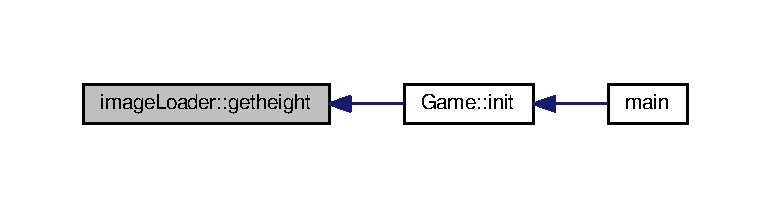
\includegraphics[width=350pt]{classimage_loader_a710984dbe3f87efd871e3ce244115ce7_icgraph}
\end{center}
\end{figure}


\hypertarget{classimage_loader_a00048f8b6d80275946c05b1b74377053}{}\index{image\+Loader@{image\+Loader}!get\+Texture@{get\+Texture}}
\index{get\+Texture@{get\+Texture}!image\+Loader@{image\+Loader}}
\subsubsection[{get\+Texture}]{\setlength{\rightskip}{0pt plus 5cm}G\+Luint image\+Loader\+::get\+Texture (
\begin{DoxyParamCaption}
{}
\end{DoxyParamCaption}
)\hspace{0.3cm}{\ttfamily [inline]}}\label{classimage_loader_a00048f8b6d80275946c05b1b74377053}


Definition at line 23 of file image\+Loader.\+h.

\hypertarget{classimage_loader_a0cd6e95e0d7aafeeb1fb6b8589c6579b}{}\index{image\+Loader@{image\+Loader}!getwidth@{getwidth}}
\index{getwidth@{getwidth}!image\+Loader@{image\+Loader}}
\subsubsection[{getwidth}]{\setlength{\rightskip}{0pt plus 5cm}int image\+Loader\+::getwidth (
\begin{DoxyParamCaption}
{}
\end{DoxyParamCaption}
)\hspace{0.3cm}{\ttfamily [inline]}}\label{classimage_loader_a0cd6e95e0d7aafeeb1fb6b8589c6579b}


Definition at line 24 of file image\+Loader.\+h.



Here is the caller graph for this function\+:\nopagebreak
\begin{figure}[H]
\begin{center}
\leavevmode
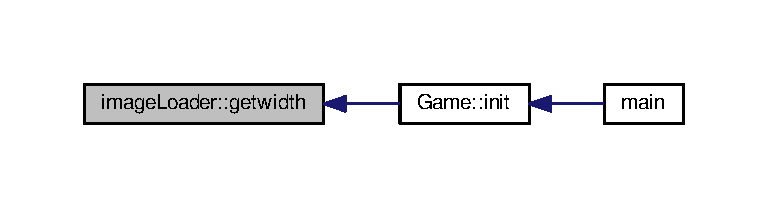
\includegraphics[width=350pt]{classimage_loader_a0cd6e95e0d7aafeeb1fb6b8589c6579b_icgraph}
\end{center}
\end{figure}


\hypertarget{classimage_loader_a15eb99f98ce36061e29d644803f4dce9}{}\index{image\+Loader@{image\+Loader}!load\+Texture@{load\+Texture}}
\index{load\+Texture@{load\+Texture}!image\+Loader@{image\+Loader}}
\subsubsection[{load\+Texture}]{\setlength{\rightskip}{0pt plus 5cm}G\+Luint image\+Loader\+::load\+Texture (
\begin{DoxyParamCaption}
\item[{std\+::string}]{path}
\end{DoxyParamCaption}
)}\label{classimage_loader_a15eb99f98ce36061e29d644803f4dce9}


Definition at line 15 of file image\+Loader.\+cpp.



Here is the caller graph for this function\+:\nopagebreak
\begin{figure}[H]
\begin{center}
\leavevmode
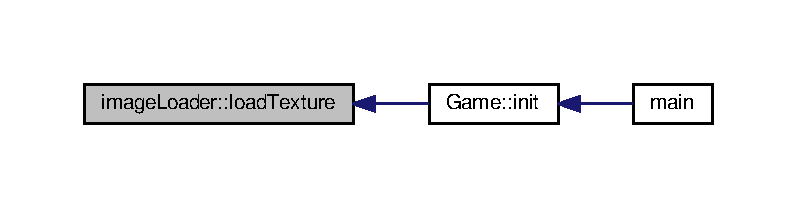
\includegraphics[width=350pt]{classimage_loader_a15eb99f98ce36061e29d644803f4dce9_icgraph}
\end{center}
\end{figure}




The documentation for this class was generated from the following files\+:\begin{DoxyCompactItemize}
\item 
\hyperlink{image_loader_8h}{image\+Loader.\+h}\item 
\hyperlink{image_loader_8cpp}{image\+Loader.\+cpp}\end{DoxyCompactItemize}

\hypertarget{class_shader}{}\section{Shader Class Reference}
\label{class_shader}\index{Shader@{Shader}}


{\ttfamily \#include $<$shader.\+h$>$}

\subsection*{Public Member Functions}
\begin{DoxyCompactItemize}
\item 
\hyperlink{class_shader_a0d654ebaca4e0555197c0724c6d30610}{Shader} ()
\item 
void \hyperlink{class_shader_a962e502d2a94b9071a20ab3c7a096104}{load\+Shader} (const G\+Lchar $\ast$vertex\+Shader\+Source, const G\+Lchar $\ast$fragment\+Shader\+Source)
\item 
void \hyperlink{class_shader_a870fa9f13d69e558815d6fd351a469dc}{use} ()
\end{DoxyCompactItemize}
\subsection*{Public Attributes}
\begin{DoxyCompactItemize}
\item 
G\+Luint \hyperlink{class_shader_af036f983d35fe0f8f31dedc009b3645e}{program}
\end{DoxyCompactItemize}


\subsection{Detailed Description}


Definition at line 11 of file shader.\+h.



\subsection{Constructor \& Destructor Documentation}
\hypertarget{class_shader_a0d654ebaca4e0555197c0724c6d30610}{}\index{Shader@{Shader}!Shader@{Shader}}
\index{Shader@{Shader}!Shader@{Shader}}
\subsubsection[{Shader}]{\setlength{\rightskip}{0pt plus 5cm}Shader\+::\+Shader (
\begin{DoxyParamCaption}
{}
\end{DoxyParamCaption}
)}\label{class_shader_a0d654ebaca4e0555197c0724c6d30610}


Definition at line 8 of file shader.\+cpp.



\subsection{Member Function Documentation}
\hypertarget{class_shader_a962e502d2a94b9071a20ab3c7a096104}{}\index{Shader@{Shader}!load\+Shader@{load\+Shader}}
\index{load\+Shader@{load\+Shader}!Shader@{Shader}}
\subsubsection[{load\+Shader}]{\setlength{\rightskip}{0pt plus 5cm}void Shader\+::load\+Shader (
\begin{DoxyParamCaption}
\item[{const G\+Lchar $\ast$}]{vertex\+Shader\+Source, }
\item[{const G\+Lchar $\ast$}]{fragment\+Shader\+Source}
\end{DoxyParamCaption}
)}\label{class_shader_a962e502d2a94b9071a20ab3c7a096104}


Definition at line 13 of file shader.\+cpp.



Here is the caller graph for this function\+:\nopagebreak
\begin{figure}[H]
\begin{center}
\leavevmode
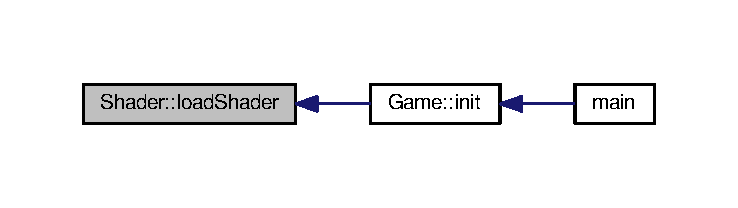
\includegraphics[width=350pt]{class_shader_a962e502d2a94b9071a20ab3c7a096104_icgraph}
\end{center}
\end{figure}


\hypertarget{class_shader_a870fa9f13d69e558815d6fd351a469dc}{}\index{Shader@{Shader}!use@{use}}
\index{use@{use}!Shader@{Shader}}
\subsubsection[{use}]{\setlength{\rightskip}{0pt plus 5cm}void Shader\+::use (
\begin{DoxyParamCaption}
{}
\end{DoxyParamCaption}
)}\label{class_shader_a870fa9f13d69e558815d6fd351a469dc}


Definition at line 80 of file shader.\+cpp.



Here is the caller graph for this function\+:\nopagebreak
\begin{figure}[H]
\begin{center}
\leavevmode
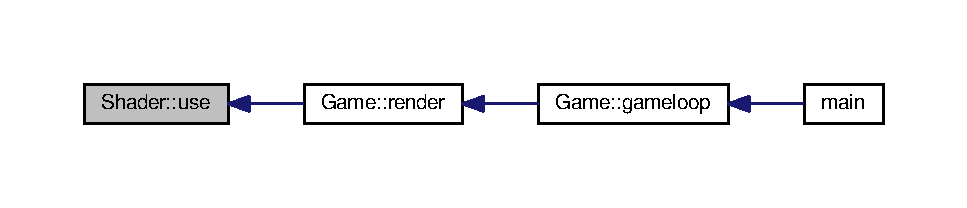
\includegraphics[width=350pt]{class_shader_a870fa9f13d69e558815d6fd351a469dc_icgraph}
\end{center}
\end{figure}




\subsection{Member Data Documentation}
\hypertarget{class_shader_af036f983d35fe0f8f31dedc009b3645e}{}\index{Shader@{Shader}!program@{program}}
\index{program@{program}!Shader@{Shader}}
\subsubsection[{program}]{\setlength{\rightskip}{0pt plus 5cm}G\+Luint Shader\+::program}\label{class_shader_af036f983d35fe0f8f31dedc009b3645e}


Definition at line 17 of file shader.\+h.



The documentation for this class was generated from the following files\+:\begin{DoxyCompactItemize}
\item 
\hyperlink{shader_8h}{shader.\+h}\item 
\hyperlink{shader_8cpp}{shader.\+cpp}\end{DoxyCompactItemize}

\hypertarget{class_time}{}\section{Time Class Reference}
\label{class_time}\index{Time@{Time}}


{\ttfamily \#include $<$Time.\+h$>$}

\subsection*{Public Member Functions}
\begin{DoxyCompactItemize}
\item 
\hyperlink{class_time_a4245e409c7347d1d671858962c2ca3b5}{Time} ()
\item 
\hyperlink{class_time_a1e92dbe963fa3cdd6bea207680f5f6d1}{$\sim$\+Time} ()
\item 
void \hyperlink{class_time_a385b4c0869ed969b266535ae835d135d}{Delta\+Time} ()
\item 
void \hyperlink{class_time_a8ccf48d1b779c21143c0a96c2574514e}{Cap\+Frame\+Rate} ()
\end{DoxyCompactItemize}
\subsection*{Public Attributes}
\begin{DoxyCompactItemize}
\item 
G\+Lfloat \hyperlink{class_time_a7dd93631e77477e08954476b0f56f013}{delta\+Time}
\item 
G\+Lfloat \hyperlink{class_time_adda8e3dcf090474f66b60ba354843270}{last\+Frame}
\item 
G\+Lfloat \hyperlink{class_time_a8f870e4dd1a743941cd40c80c3dc86e0}{current\+Frame}
\item 
int \hyperlink{class_time_a1ea63396edff67d5069ab9dd2e8f3c44}{max\+F\+P\+S}
\end{DoxyCompactItemize}


\subsection{Detailed Description}
Class to limit and control frame rate / camera movement speed, or aleast atempt to. Never quite got the {\ttfamily Deltatime()} function to work correctly. 

Definition at line 14 of file Time.\+h.



\subsection{Constructor \& Destructor Documentation}
\hypertarget{class_time_a4245e409c7347d1d671858962c2ca3b5}{}\index{Time@{Time}!Time@{Time}}
\index{Time@{Time}!Time@{Time}}
\subsubsection[{Time}]{\setlength{\rightskip}{0pt plus 5cm}Time\+::\+Time (
\begin{DoxyParamCaption}
{}
\end{DoxyParamCaption}
)}\label{class_time_a4245e409c7347d1d671858962c2ca3b5}


Definition at line 3 of file Time.\+cpp.

\hypertarget{class_time_a1e92dbe963fa3cdd6bea207680f5f6d1}{}\index{Time@{Time}!````~Time@{$\sim$\+Time}}
\index{````~Time@{$\sim$\+Time}!Time@{Time}}
\subsubsection[{$\sim$\+Time}]{\setlength{\rightskip}{0pt plus 5cm}Time\+::$\sim$\+Time (
\begin{DoxyParamCaption}
{}
\end{DoxyParamCaption}
)}\label{class_time_a1e92dbe963fa3cdd6bea207680f5f6d1}


Definition at line 11 of file Time.\+cpp.



\subsection{Member Function Documentation}
\hypertarget{class_time_a8ccf48d1b779c21143c0a96c2574514e}{}\index{Time@{Time}!Cap\+Frame\+Rate@{Cap\+Frame\+Rate}}
\index{Cap\+Frame\+Rate@{Cap\+Frame\+Rate}!Time@{Time}}
\subsubsection[{Cap\+Frame\+Rate}]{\setlength{\rightskip}{0pt plus 5cm}void Time\+::\+Cap\+Frame\+Rate (
\begin{DoxyParamCaption}
{}
\end{DoxyParamCaption}
)}\label{class_time_a8ccf48d1b779c21143c0a96c2574514e}
Basic frame rate cap. 

Definition at line 26 of file Time.\+cpp.



Here is the caller graph for this function\+:\nopagebreak
\begin{figure}[H]
\begin{center}
\leavevmode
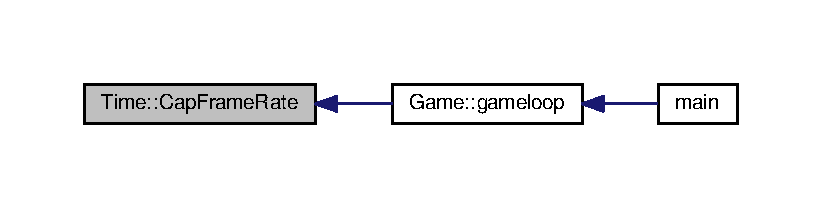
\includegraphics[width=350pt]{class_time_a8ccf48d1b779c21143c0a96c2574514e_icgraph}
\end{center}
\end{figure}


\hypertarget{class_time_a385b4c0869ed969b266535ae835d135d}{}\index{Time@{Time}!Delta\+Time@{Delta\+Time}}
\index{Delta\+Time@{Delta\+Time}!Time@{Time}}
\subsubsection[{Delta\+Time}]{\setlength{\rightskip}{0pt plus 5cm}void Time\+::\+Delta\+Time (
\begin{DoxyParamCaption}
{}
\end{DoxyParamCaption}
)}\label{class_time_a385b4c0869ed969b266535ae835d135d}
\begin{DoxyRefDesc}{Bug}
\item[\hyperlink{bug__bug000002}{Bug}]Does not wotk as expected. Wanted a function that would act like Unity3ds Time.\+deltatime \end{DoxyRefDesc}


Definition at line 17 of file Time.\+cpp.



Here is the caller graph for this function\+:\nopagebreak
\begin{figure}[H]
\begin{center}
\leavevmode
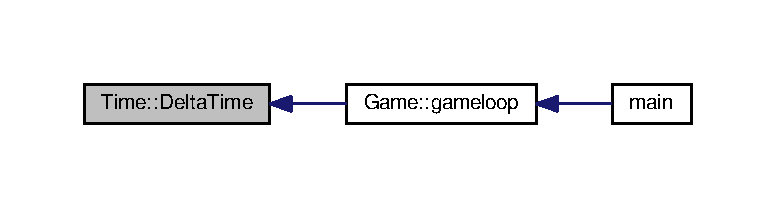
\includegraphics[width=350pt]{class_time_a385b4c0869ed969b266535ae835d135d_icgraph}
\end{center}
\end{figure}




\subsection{Member Data Documentation}
\hypertarget{class_time_a8f870e4dd1a743941cd40c80c3dc86e0}{}\index{Time@{Time}!current\+Frame@{current\+Frame}}
\index{current\+Frame@{current\+Frame}!Time@{Time}}
\subsubsection[{current\+Frame}]{\setlength{\rightskip}{0pt plus 5cm}G\+Lfloat Time\+::current\+Frame}\label{class_time_a8f870e4dd1a743941cd40c80c3dc86e0}


Definition at line 26 of file Time.\+h.

\hypertarget{class_time_a7dd93631e77477e08954476b0f56f013}{}\index{Time@{Time}!delta\+Time@{delta\+Time}}
\index{delta\+Time@{delta\+Time}!Time@{Time}}
\subsubsection[{delta\+Time}]{\setlength{\rightskip}{0pt plus 5cm}G\+Lfloat Time\+::delta\+Time}\label{class_time_a7dd93631e77477e08954476b0f56f013}


Definition at line 23 of file Time.\+h.

\hypertarget{class_time_adda8e3dcf090474f66b60ba354843270}{}\index{Time@{Time}!last\+Frame@{last\+Frame}}
\index{last\+Frame@{last\+Frame}!Time@{Time}}
\subsubsection[{last\+Frame}]{\setlength{\rightskip}{0pt plus 5cm}G\+Lfloat Time\+::last\+Frame}\label{class_time_adda8e3dcf090474f66b60ba354843270}


Definition at line 24 of file Time.\+h.

\hypertarget{class_time_a1ea63396edff67d5069ab9dd2e8f3c44}{}\index{Time@{Time}!max\+F\+P\+S@{max\+F\+P\+S}}
\index{max\+F\+P\+S@{max\+F\+P\+S}!Time@{Time}}
\subsubsection[{max\+F\+P\+S}]{\setlength{\rightskip}{0pt plus 5cm}int Time\+::max\+F\+P\+S}\label{class_time_a1ea63396edff67d5069ab9dd2e8f3c44}


Definition at line 27 of file Time.\+h.



The documentation for this class was generated from the following files\+:\begin{DoxyCompactItemize}
\item 
\hyperlink{_time_8h}{Time.\+h}\item 
\hyperlink{_time_8cpp}{Time.\+cpp}\end{DoxyCompactItemize}

\chapter{File Documentation}
\hypertarget{_c_make_c_compiler_id_8c}{}\section{build/\+C\+Make\+Files/2.8.12.2/\+Compiler\+Id\+C/\+C\+Make\+C\+Compiler\+Id.c File Reference}
\label{_c_make_c_compiler_id_8c}\index{build/\+C\+Make\+Files/2.\+8.\+12.\+2/\+Compiler\+Id\+C/\+C\+Make\+C\+Compiler\+Id.\+c@{build/\+C\+Make\+Files/2.\+8.\+12.\+2/\+Compiler\+Id\+C/\+C\+Make\+C\+Compiler\+Id.\+c}}
\subsection*{Macros}
\begin{DoxyCompactItemize}
\item 
\#define \hyperlink{_c_make_c_compiler_id_8c_a81dee0709ded976b2e0319239f72d174}{C\+O\+M\+P\+I\+L\+E\+R\+\_\+\+I\+D}~\char`\"{}\char`\"{}
\item 
\#define \hyperlink{_c_make_c_compiler_id_8c_adbc5372f40838899018fadbc89bd588b}{P\+L\+A\+T\+F\+O\+R\+M\+\_\+\+I\+D}~\char`\"{}\char`\"{}
\item 
\#define \hyperlink{_c_make_c_compiler_id_8c_aba35d0d200deaeb06aee95ca297acb28}{A\+R\+C\+H\+I\+T\+E\+C\+T\+U\+R\+E\+\_\+\+I\+D}~\char`\"{}\char`\"{}
\item 
\#define \hyperlink{_c_make_c_compiler_id_8c_ad1280362da42492bbc11aa78cbf776ad}{D\+E\+C}(n)
\item 
\#define \hyperlink{_c_make_c_compiler_id_8c_a46d5d95daa1bef867bd0179594310ed5}{H\+E\+X}(n)
\end{DoxyCompactItemize}
\subsection*{Functions}
\begin{DoxyCompactItemize}
\item 
int \hyperlink{_c_make_c_compiler_id_8c_a0ddf1224851353fc92bfbff6f499fa97}{main} (int argc, char $\ast$argv\mbox{[}$\,$\mbox{]})
\end{DoxyCompactItemize}
\subsection*{Variables}
\begin{DoxyCompactItemize}
\item 
char const $\ast$ \hyperlink{_c_make_c_compiler_id_8c_a4b0efeb7a5d59313986b3a0390f050f6}{info\+\_\+compiler} = \char`\"{}I\+N\+F\+O\char`\"{} \char`\"{}\+:\char`\"{} \char`\"{}compiler\mbox{[}\char`\"{} C\+O\+M\+P\+I\+L\+E\+R\+\_\+\+I\+D \char`\"{}\mbox{]}\char`\"{}
\item 
char const $\ast$ \hyperlink{_c_make_c_compiler_id_8c_a2321403dee54ee23f0c2fa849c60f7d4}{info\+\_\+platform} = \char`\"{}I\+N\+F\+O\char`\"{} \char`\"{}\+:\char`\"{} \char`\"{}platform\mbox{[}\char`\"{} P\+L\+A\+T\+F\+O\+R\+M\+\_\+\+I\+D \char`\"{}\mbox{]}\char`\"{}
\item 
char const $\ast$ \hyperlink{_c_make_c_compiler_id_8c_a59647e99d304ed33b15cb284c27ed391}{info\+\_\+arch} = \char`\"{}I\+N\+F\+O\char`\"{} \char`\"{}\+:\char`\"{} \char`\"{}arch\mbox{[}\char`\"{} A\+R\+C\+H\+I\+T\+E\+C\+T\+U\+R\+E\+\_\+\+I\+D \char`\"{}\mbox{]}\char`\"{}
\end{DoxyCompactItemize}


\subsection{Macro Definition Documentation}
\hypertarget{_c_make_c_compiler_id_8c_aba35d0d200deaeb06aee95ca297acb28}{}\index{C\+Make\+C\+Compiler\+Id.\+c@{C\+Make\+C\+Compiler\+Id.\+c}!A\+R\+C\+H\+I\+T\+E\+C\+T\+U\+R\+E\+\_\+\+I\+D@{A\+R\+C\+H\+I\+T\+E\+C\+T\+U\+R\+E\+\_\+\+I\+D}}
\index{A\+R\+C\+H\+I\+T\+E\+C\+T\+U\+R\+E\+\_\+\+I\+D@{A\+R\+C\+H\+I\+T\+E\+C\+T\+U\+R\+E\+\_\+\+I\+D}!C\+Make\+C\+Compiler\+Id.\+c@{C\+Make\+C\+Compiler\+Id.\+c}}
\subsubsection[{A\+R\+C\+H\+I\+T\+E\+C\+T\+U\+R\+E\+\_\+\+I\+D}]{\setlength{\rightskip}{0pt plus 5cm}\#define A\+R\+C\+H\+I\+T\+E\+C\+T\+U\+R\+E\+\_\+\+I\+D~\char`\"{}\char`\"{}}\label{_c_make_c_compiler_id_8c_aba35d0d200deaeb06aee95ca297acb28}


Definition at line 320 of file C\+Make\+C\+Compiler\+Id.\+c.

\hypertarget{_c_make_c_compiler_id_8c_a81dee0709ded976b2e0319239f72d174}{}\index{C\+Make\+C\+Compiler\+Id.\+c@{C\+Make\+C\+Compiler\+Id.\+c}!C\+O\+M\+P\+I\+L\+E\+R\+\_\+\+I\+D@{C\+O\+M\+P\+I\+L\+E\+R\+\_\+\+I\+D}}
\index{C\+O\+M\+P\+I\+L\+E\+R\+\_\+\+I\+D@{C\+O\+M\+P\+I\+L\+E\+R\+\_\+\+I\+D}!C\+Make\+C\+Compiler\+Id.\+c@{C\+Make\+C\+Compiler\+Id.\+c}}
\subsubsection[{C\+O\+M\+P\+I\+L\+E\+R\+\_\+\+I\+D}]{\setlength{\rightskip}{0pt plus 5cm}\#define C\+O\+M\+P\+I\+L\+E\+R\+\_\+\+I\+D~\char`\"{}\char`\"{}}\label{_c_make_c_compiler_id_8c_a81dee0709ded976b2e0319239f72d174}


Definition at line 200 of file C\+Make\+C\+Compiler\+Id.\+c.

\hypertarget{_c_make_c_compiler_id_8c_ad1280362da42492bbc11aa78cbf776ad}{}\index{C\+Make\+C\+Compiler\+Id.\+c@{C\+Make\+C\+Compiler\+Id.\+c}!D\+E\+C@{D\+E\+C}}
\index{D\+E\+C@{D\+E\+C}!C\+Make\+C\+Compiler\+Id.\+c@{C\+Make\+C\+Compiler\+Id.\+c}}
\subsubsection[{D\+E\+C}]{\setlength{\rightskip}{0pt plus 5cm}\#define D\+E\+C(
\begin{DoxyParamCaption}
\item[{}]{n}
\end{DoxyParamCaption}
)}\label{_c_make_c_compiler_id_8c_ad1280362da42492bbc11aa78cbf776ad}
{\bfseries Value\+:}
\begin{DoxyCode}
(\textcolor{charliteral}{'0'} + (((n) / 10000000)%10)), \(\backslash\)
  (\textcolor{charliteral}{'0'} + (((n) / 1000000)%10)),  \(\backslash\)
  (\textcolor{charliteral}{'0'} + (((n) / 100000)%10)),   \(\backslash\)
  (\textcolor{charliteral}{'0'} + (((n) / 10000)%10)),    \(\backslash\)
  (\textcolor{charliteral}{'0'} + (((n) / 1000)%10)),     \(\backslash\)
  (\textcolor{charliteral}{'0'} + (((n) / 100)%10)),      \(\backslash\)
  (\textcolor{charliteral}{'0'} + (((n) / 10)%10)),       \(\backslash\)
  (\textcolor{charliteral}{'0'} +  ((n) % 10))
\end{DoxyCode}


Definition at line 324 of file C\+Make\+C\+Compiler\+Id.\+c.

\hypertarget{_c_make_c_compiler_id_8c_a46d5d95daa1bef867bd0179594310ed5}{}\index{C\+Make\+C\+Compiler\+Id.\+c@{C\+Make\+C\+Compiler\+Id.\+c}!H\+E\+X@{H\+E\+X}}
\index{H\+E\+X@{H\+E\+X}!C\+Make\+C\+Compiler\+Id.\+c@{C\+Make\+C\+Compiler\+Id.\+c}}
\subsubsection[{H\+E\+X}]{\setlength{\rightskip}{0pt plus 5cm}\#define H\+E\+X(
\begin{DoxyParamCaption}
\item[{}]{n}
\end{DoxyParamCaption}
)}\label{_c_make_c_compiler_id_8c_a46d5d95daa1bef867bd0179594310ed5}
{\bfseries Value\+:}
\begin{DoxyCode}
(\textcolor{charliteral}{'0'} + ((n)>>28 & 0xF)), \(\backslash\)
  (\textcolor{charliteral}{'0'} + ((n)>>24 & 0xF)), \(\backslash\)
  (\textcolor{charliteral}{'0'} + ((n)>>20 & 0xF)), \(\backslash\)
  (\textcolor{charliteral}{'0'} + ((n)>>16 & 0xF)), \(\backslash\)
  (\textcolor{charliteral}{'0'} + ((n)>>12 & 0xF)), \(\backslash\)
  (\textcolor{charliteral}{'0'} + ((n)>>8  & 0xF)), \(\backslash\)
  (\textcolor{charliteral}{'0'} + ((n)>>4  & 0xF)), \(\backslash\)
  (\textcolor{charliteral}{'0'} + ((n)     & 0xF))
\end{DoxyCode}


Definition at line 335 of file C\+Make\+C\+Compiler\+Id.\+c.

\hypertarget{_c_make_c_compiler_id_8c_adbc5372f40838899018fadbc89bd588b}{}\index{C\+Make\+C\+Compiler\+Id.\+c@{C\+Make\+C\+Compiler\+Id.\+c}!P\+L\+A\+T\+F\+O\+R\+M\+\_\+\+I\+D@{P\+L\+A\+T\+F\+O\+R\+M\+\_\+\+I\+D}}
\index{P\+L\+A\+T\+F\+O\+R\+M\+\_\+\+I\+D@{P\+L\+A\+T\+F\+O\+R\+M\+\_\+\+I\+D}!C\+Make\+C\+Compiler\+Id.\+c@{C\+Make\+C\+Compiler\+Id.\+c}}
\subsubsection[{P\+L\+A\+T\+F\+O\+R\+M\+\_\+\+I\+D}]{\setlength{\rightskip}{0pt plus 5cm}\#define P\+L\+A\+T\+F\+O\+R\+M\+\_\+\+I\+D~\char`\"{}\char`\"{}}\label{_c_make_c_compiler_id_8c_adbc5372f40838899018fadbc89bd588b}


Definition at line 287 of file C\+Make\+C\+Compiler\+Id.\+c.



\subsection{Function Documentation}
\hypertarget{_c_make_c_compiler_id_8c_a0ddf1224851353fc92bfbff6f499fa97}{}\index{C\+Make\+C\+Compiler\+Id.\+c@{C\+Make\+C\+Compiler\+Id.\+c}!main@{main}}
\index{main@{main}!C\+Make\+C\+Compiler\+Id.\+c@{C\+Make\+C\+Compiler\+Id.\+c}}
\subsubsection[{main}]{\setlength{\rightskip}{0pt plus 5cm}int main (
\begin{DoxyParamCaption}
\item[{int}]{argc, }
\item[{char $\ast$}]{argv\mbox{[}$\,$\mbox{]}}
\end{DoxyParamCaption}
)}\label{_c_make_c_compiler_id_8c_a0ddf1224851353fc92bfbff6f499fa97}


Definition at line 377 of file C\+Make\+C\+Compiler\+Id.\+c.



\subsection{Variable Documentation}
\hypertarget{_c_make_c_compiler_id_8c_a59647e99d304ed33b15cb284c27ed391}{}\index{C\+Make\+C\+Compiler\+Id.\+c@{C\+Make\+C\+Compiler\+Id.\+c}!info\+\_\+arch@{info\+\_\+arch}}
\index{info\+\_\+arch@{info\+\_\+arch}!C\+Make\+C\+Compiler\+Id.\+c@{C\+Make\+C\+Compiler\+Id.\+c}}
\subsubsection[{info\+\_\+arch}]{\setlength{\rightskip}{0pt plus 5cm}char const$\ast$ info\+\_\+arch = \char`\"{}I\+N\+F\+O\char`\"{} \char`\"{}\+:\char`\"{} \char`\"{}arch\mbox{[}\char`\"{} A\+R\+C\+H\+I\+T\+E\+C\+T\+U\+R\+E\+\_\+\+I\+D \char`\"{}\mbox{]}\char`\"{}}\label{_c_make_c_compiler_id_8c_a59647e99d304ed33b15cb284c27ed391}


Definition at line 368 of file C\+Make\+C\+Compiler\+Id.\+c.

\hypertarget{_c_make_c_compiler_id_8c_a4b0efeb7a5d59313986b3a0390f050f6}{}\index{C\+Make\+C\+Compiler\+Id.\+c@{C\+Make\+C\+Compiler\+Id.\+c}!info\+\_\+compiler@{info\+\_\+compiler}}
\index{info\+\_\+compiler@{info\+\_\+compiler}!C\+Make\+C\+Compiler\+Id.\+c@{C\+Make\+C\+Compiler\+Id.\+c}}
\subsubsection[{info\+\_\+compiler}]{\setlength{\rightskip}{0pt plus 5cm}char const$\ast$ info\+\_\+compiler = \char`\"{}I\+N\+F\+O\char`\"{} \char`\"{}\+:\char`\"{} \char`\"{}compiler\mbox{[}\char`\"{} C\+O\+M\+P\+I\+L\+E\+R\+\_\+\+I\+D \char`\"{}\mbox{]}\char`\"{}}\label{_c_make_c_compiler_id_8c_a4b0efeb7a5d59313986b3a0390f050f6}


Definition at line 208 of file C\+Make\+C\+Compiler\+Id.\+c.

\hypertarget{_c_make_c_compiler_id_8c_a2321403dee54ee23f0c2fa849c60f7d4}{}\index{C\+Make\+C\+Compiler\+Id.\+c@{C\+Make\+C\+Compiler\+Id.\+c}!info\+\_\+platform@{info\+\_\+platform}}
\index{info\+\_\+platform@{info\+\_\+platform}!C\+Make\+C\+Compiler\+Id.\+c@{C\+Make\+C\+Compiler\+Id.\+c}}
\subsubsection[{info\+\_\+platform}]{\setlength{\rightskip}{0pt plus 5cm}char const$\ast$ info\+\_\+platform = \char`\"{}I\+N\+F\+O\char`\"{} \char`\"{}\+:\char`\"{} \char`\"{}platform\mbox{[}\char`\"{} P\+L\+A\+T\+F\+O\+R\+M\+\_\+\+I\+D \char`\"{}\mbox{]}\char`\"{}}\label{_c_make_c_compiler_id_8c_a2321403dee54ee23f0c2fa849c60f7d4}


Definition at line 367 of file C\+Make\+C\+Compiler\+Id.\+c.


\hypertarget{_c_make_c_x_x_compiler_id_8cpp}{}\section{build/\+C\+Make\+Files/2.8.12.2/\+Compiler\+Id\+C\+X\+X/\+C\+Make\+C\+X\+X\+Compiler\+Id.cpp File Reference}
\label{_c_make_c_x_x_compiler_id_8cpp}\index{build/\+C\+Make\+Files/2.\+8.\+12.\+2/\+Compiler\+Id\+C\+X\+X/\+C\+Make\+C\+X\+X\+Compiler\+Id.\+cpp@{build/\+C\+Make\+Files/2.\+8.\+12.\+2/\+Compiler\+Id\+C\+X\+X/\+C\+Make\+C\+X\+X\+Compiler\+Id.\+cpp}}
\subsection*{Macros}
\begin{DoxyCompactItemize}
\item 
\#define \hyperlink{_c_make_c_x_x_compiler_id_8cpp_a81dee0709ded976b2e0319239f72d174}{C\+O\+M\+P\+I\+L\+E\+R\+\_\+\+I\+D}~\char`\"{}\char`\"{}
\item 
\#define \hyperlink{_c_make_c_x_x_compiler_id_8cpp_adbc5372f40838899018fadbc89bd588b}{P\+L\+A\+T\+F\+O\+R\+M\+\_\+\+I\+D}~\char`\"{}\char`\"{}
\item 
\#define \hyperlink{_c_make_c_x_x_compiler_id_8cpp_aba35d0d200deaeb06aee95ca297acb28}{A\+R\+C\+H\+I\+T\+E\+C\+T\+U\+R\+E\+\_\+\+I\+D}~\char`\"{}\char`\"{}
\item 
\#define \hyperlink{_c_make_c_x_x_compiler_id_8cpp_ad1280362da42492bbc11aa78cbf776ad}{D\+E\+C}(n)
\item 
\#define \hyperlink{_c_make_c_x_x_compiler_id_8cpp_a46d5d95daa1bef867bd0179594310ed5}{H\+E\+X}(n)
\end{DoxyCompactItemize}
\subsection*{Functions}
\begin{DoxyCompactItemize}
\item 
int \hyperlink{_c_make_c_x_x_compiler_id_8cpp_a0ddf1224851353fc92bfbff6f499fa97}{main} (int argc, char $\ast$argv\mbox{[}$\,$\mbox{]})
\end{DoxyCompactItemize}
\subsection*{Variables}
\begin{DoxyCompactItemize}
\item 
char const $\ast$ \hyperlink{_c_make_c_x_x_compiler_id_8cpp_a4b0efeb7a5d59313986b3a0390f050f6}{info\+\_\+compiler} = \char`\"{}I\+N\+F\+O\char`\"{} \char`\"{}\+:\char`\"{} \char`\"{}compiler\mbox{[}\char`\"{} C\+O\+M\+P\+I\+L\+E\+R\+\_\+\+I\+D \char`\"{}\mbox{]}\char`\"{}
\item 
char const $\ast$ \hyperlink{_c_make_c_x_x_compiler_id_8cpp_a2321403dee54ee23f0c2fa849c60f7d4}{info\+\_\+platform} = \char`\"{}I\+N\+F\+O\char`\"{} \char`\"{}\+:\char`\"{} \char`\"{}platform\mbox{[}\char`\"{} P\+L\+A\+T\+F\+O\+R\+M\+\_\+\+I\+D \char`\"{}\mbox{]}\char`\"{}
\item 
char const $\ast$ \hyperlink{_c_make_c_x_x_compiler_id_8cpp_a59647e99d304ed33b15cb284c27ed391}{info\+\_\+arch} = \char`\"{}I\+N\+F\+O\char`\"{} \char`\"{}\+:\char`\"{} \char`\"{}arch\mbox{[}\char`\"{} A\+R\+C\+H\+I\+T\+E\+C\+T\+U\+R\+E\+\_\+\+I\+D \char`\"{}\mbox{]}\char`\"{}
\end{DoxyCompactItemize}


\subsection{Macro Definition Documentation}
\hypertarget{_c_make_c_x_x_compiler_id_8cpp_aba35d0d200deaeb06aee95ca297acb28}{}\index{C\+Make\+C\+X\+X\+Compiler\+Id.\+cpp@{C\+Make\+C\+X\+X\+Compiler\+Id.\+cpp}!A\+R\+C\+H\+I\+T\+E\+C\+T\+U\+R\+E\+\_\+\+I\+D@{A\+R\+C\+H\+I\+T\+E\+C\+T\+U\+R\+E\+\_\+\+I\+D}}
\index{A\+R\+C\+H\+I\+T\+E\+C\+T\+U\+R\+E\+\_\+\+I\+D@{A\+R\+C\+H\+I\+T\+E\+C\+T\+U\+R\+E\+\_\+\+I\+D}!C\+Make\+C\+X\+X\+Compiler\+Id.\+cpp@{C\+Make\+C\+X\+X\+Compiler\+Id.\+cpp}}
\subsubsection[{A\+R\+C\+H\+I\+T\+E\+C\+T\+U\+R\+E\+\_\+\+I\+D}]{\setlength{\rightskip}{0pt plus 5cm}\#define A\+R\+C\+H\+I\+T\+E\+C\+T\+U\+R\+E\+\_\+\+I\+D~\char`\"{}\char`\"{}}\label{_c_make_c_x_x_compiler_id_8cpp_aba35d0d200deaeb06aee95ca297acb28}


Definition at line 313 of file C\+Make\+C\+X\+X\+Compiler\+Id.\+cpp.

\hypertarget{_c_make_c_x_x_compiler_id_8cpp_a81dee0709ded976b2e0319239f72d174}{}\index{C\+Make\+C\+X\+X\+Compiler\+Id.\+cpp@{C\+Make\+C\+X\+X\+Compiler\+Id.\+cpp}!C\+O\+M\+P\+I\+L\+E\+R\+\_\+\+I\+D@{C\+O\+M\+P\+I\+L\+E\+R\+\_\+\+I\+D}}
\index{C\+O\+M\+P\+I\+L\+E\+R\+\_\+\+I\+D@{C\+O\+M\+P\+I\+L\+E\+R\+\_\+\+I\+D}!C\+Make\+C\+X\+X\+Compiler\+Id.\+cpp@{C\+Make\+C\+X\+X\+Compiler\+Id.\+cpp}}
\subsubsection[{C\+O\+M\+P\+I\+L\+E\+R\+\_\+\+I\+D}]{\setlength{\rightskip}{0pt plus 5cm}\#define C\+O\+M\+P\+I\+L\+E\+R\+\_\+\+I\+D~\char`\"{}\char`\"{}}\label{_c_make_c_x_x_compiler_id_8cpp_a81dee0709ded976b2e0319239f72d174}


Definition at line 193 of file C\+Make\+C\+X\+X\+Compiler\+Id.\+cpp.

\hypertarget{_c_make_c_x_x_compiler_id_8cpp_ad1280362da42492bbc11aa78cbf776ad}{}\index{C\+Make\+C\+X\+X\+Compiler\+Id.\+cpp@{C\+Make\+C\+X\+X\+Compiler\+Id.\+cpp}!D\+E\+C@{D\+E\+C}}
\index{D\+E\+C@{D\+E\+C}!C\+Make\+C\+X\+X\+Compiler\+Id.\+cpp@{C\+Make\+C\+X\+X\+Compiler\+Id.\+cpp}}
\subsubsection[{D\+E\+C}]{\setlength{\rightskip}{0pt plus 5cm}\#define D\+E\+C(
\begin{DoxyParamCaption}
\item[{}]{n}
\end{DoxyParamCaption}
)}\label{_c_make_c_x_x_compiler_id_8cpp_ad1280362da42492bbc11aa78cbf776ad}
{\bfseries Value\+:}
\begin{DoxyCode}
(\textcolor{charliteral}{'0'} + (((n) / 10000000)%10)), \(\backslash\)
  (\textcolor{charliteral}{'0'} + (((n) / 1000000)%10)),  \(\backslash\)
  (\textcolor{charliteral}{'0'} + (((n) / 100000)%10)),   \(\backslash\)
  (\textcolor{charliteral}{'0'} + (((n) / 10000)%10)),    \(\backslash\)
  (\textcolor{charliteral}{'0'} + (((n) / 1000)%10)),     \(\backslash\)
  (\textcolor{charliteral}{'0'} + (((n) / 100)%10)),      \(\backslash\)
  (\textcolor{charliteral}{'0'} + (((n) / 10)%10)),       \(\backslash\)
  (\textcolor{charliteral}{'0'} +  ((n) % 10))
\end{DoxyCode}


Definition at line 317 of file C\+Make\+C\+X\+X\+Compiler\+Id.\+cpp.

\hypertarget{_c_make_c_x_x_compiler_id_8cpp_a46d5d95daa1bef867bd0179594310ed5}{}\index{C\+Make\+C\+X\+X\+Compiler\+Id.\+cpp@{C\+Make\+C\+X\+X\+Compiler\+Id.\+cpp}!H\+E\+X@{H\+E\+X}}
\index{H\+E\+X@{H\+E\+X}!C\+Make\+C\+X\+X\+Compiler\+Id.\+cpp@{C\+Make\+C\+X\+X\+Compiler\+Id.\+cpp}}
\subsubsection[{H\+E\+X}]{\setlength{\rightskip}{0pt plus 5cm}\#define H\+E\+X(
\begin{DoxyParamCaption}
\item[{}]{n}
\end{DoxyParamCaption}
)}\label{_c_make_c_x_x_compiler_id_8cpp_a46d5d95daa1bef867bd0179594310ed5}
{\bfseries Value\+:}
\begin{DoxyCode}
(\textcolor{charliteral}{'0'} + ((n)>>28 & 0xF)), \(\backslash\)
  (\textcolor{charliteral}{'0'} + ((n)>>24 & 0xF)), \(\backslash\)
  (\textcolor{charliteral}{'0'} + ((n)>>20 & 0xF)), \(\backslash\)
  (\textcolor{charliteral}{'0'} + ((n)>>16 & 0xF)), \(\backslash\)
  (\textcolor{charliteral}{'0'} + ((n)>>12 & 0xF)), \(\backslash\)
  (\textcolor{charliteral}{'0'} + ((n)>>8  & 0xF)), \(\backslash\)
  (\textcolor{charliteral}{'0'} + ((n)>>4  & 0xF)), \(\backslash\)
  (\textcolor{charliteral}{'0'} + ((n)     & 0xF))
\end{DoxyCode}


Definition at line 328 of file C\+Make\+C\+X\+X\+Compiler\+Id.\+cpp.

\hypertarget{_c_make_c_x_x_compiler_id_8cpp_adbc5372f40838899018fadbc89bd588b}{}\index{C\+Make\+C\+X\+X\+Compiler\+Id.\+cpp@{C\+Make\+C\+X\+X\+Compiler\+Id.\+cpp}!P\+L\+A\+T\+F\+O\+R\+M\+\_\+\+I\+D@{P\+L\+A\+T\+F\+O\+R\+M\+\_\+\+I\+D}}
\index{P\+L\+A\+T\+F\+O\+R\+M\+\_\+\+I\+D@{P\+L\+A\+T\+F\+O\+R\+M\+\_\+\+I\+D}!C\+Make\+C\+X\+X\+Compiler\+Id.\+cpp@{C\+Make\+C\+X\+X\+Compiler\+Id.\+cpp}}
\subsubsection[{P\+L\+A\+T\+F\+O\+R\+M\+\_\+\+I\+D}]{\setlength{\rightskip}{0pt plus 5cm}\#define P\+L\+A\+T\+F\+O\+R\+M\+\_\+\+I\+D~\char`\"{}\char`\"{}}\label{_c_make_c_x_x_compiler_id_8cpp_adbc5372f40838899018fadbc89bd588b}


Definition at line 280 of file C\+Make\+C\+X\+X\+Compiler\+Id.\+cpp.



\subsection{Function Documentation}
\hypertarget{_c_make_c_x_x_compiler_id_8cpp_a0ddf1224851353fc92bfbff6f499fa97}{}\index{C\+Make\+C\+X\+X\+Compiler\+Id.\+cpp@{C\+Make\+C\+X\+X\+Compiler\+Id.\+cpp}!main@{main}}
\index{main@{main}!C\+Make\+C\+X\+X\+Compiler\+Id.\+cpp@{C\+Make\+C\+X\+X\+Compiler\+Id.\+cpp}}
\subsubsection[{main}]{\setlength{\rightskip}{0pt plus 5cm}int main (
\begin{DoxyParamCaption}
\item[{int}]{argc, }
\item[{char $\ast$}]{argv\mbox{[}$\,$\mbox{]}}
\end{DoxyParamCaption}
)}\label{_c_make_c_x_x_compiler_id_8cpp_a0ddf1224851353fc92bfbff6f499fa97}


Definition at line 367 of file C\+Make\+C\+X\+X\+Compiler\+Id.\+cpp.



\subsection{Variable Documentation}
\hypertarget{_c_make_c_x_x_compiler_id_8cpp_a59647e99d304ed33b15cb284c27ed391}{}\index{C\+Make\+C\+X\+X\+Compiler\+Id.\+cpp@{C\+Make\+C\+X\+X\+Compiler\+Id.\+cpp}!info\+\_\+arch@{info\+\_\+arch}}
\index{info\+\_\+arch@{info\+\_\+arch}!C\+Make\+C\+X\+X\+Compiler\+Id.\+cpp@{C\+Make\+C\+X\+X\+Compiler\+Id.\+cpp}}
\subsubsection[{info\+\_\+arch}]{\setlength{\rightskip}{0pt plus 5cm}char const$\ast$ info\+\_\+arch = \char`\"{}I\+N\+F\+O\char`\"{} \char`\"{}\+:\char`\"{} \char`\"{}arch\mbox{[}\char`\"{} A\+R\+C\+H\+I\+T\+E\+C\+T\+U\+R\+E\+\_\+\+I\+D \char`\"{}\mbox{]}\char`\"{}}\label{_c_make_c_x_x_compiler_id_8cpp_a59647e99d304ed33b15cb284c27ed391}


Definition at line 361 of file C\+Make\+C\+X\+X\+Compiler\+Id.\+cpp.

\hypertarget{_c_make_c_x_x_compiler_id_8cpp_a4b0efeb7a5d59313986b3a0390f050f6}{}\index{C\+Make\+C\+X\+X\+Compiler\+Id.\+cpp@{C\+Make\+C\+X\+X\+Compiler\+Id.\+cpp}!info\+\_\+compiler@{info\+\_\+compiler}}
\index{info\+\_\+compiler@{info\+\_\+compiler}!C\+Make\+C\+X\+X\+Compiler\+Id.\+cpp@{C\+Make\+C\+X\+X\+Compiler\+Id.\+cpp}}
\subsubsection[{info\+\_\+compiler}]{\setlength{\rightskip}{0pt plus 5cm}char const$\ast$ info\+\_\+compiler = \char`\"{}I\+N\+F\+O\char`\"{} \char`\"{}\+:\char`\"{} \char`\"{}compiler\mbox{[}\char`\"{} C\+O\+M\+P\+I\+L\+E\+R\+\_\+\+I\+D \char`\"{}\mbox{]}\char`\"{}}\label{_c_make_c_x_x_compiler_id_8cpp_a4b0efeb7a5d59313986b3a0390f050f6}


Definition at line 201 of file C\+Make\+C\+X\+X\+Compiler\+Id.\+cpp.

\hypertarget{_c_make_c_x_x_compiler_id_8cpp_a2321403dee54ee23f0c2fa849c60f7d4}{}\index{C\+Make\+C\+X\+X\+Compiler\+Id.\+cpp@{C\+Make\+C\+X\+X\+Compiler\+Id.\+cpp}!info\+\_\+platform@{info\+\_\+platform}}
\index{info\+\_\+platform@{info\+\_\+platform}!C\+Make\+C\+X\+X\+Compiler\+Id.\+cpp@{C\+Make\+C\+X\+X\+Compiler\+Id.\+cpp}}
\subsubsection[{info\+\_\+platform}]{\setlength{\rightskip}{0pt plus 5cm}char const$\ast$ info\+\_\+platform = \char`\"{}I\+N\+F\+O\char`\"{} \char`\"{}\+:\char`\"{} \char`\"{}platform\mbox{[}\char`\"{} P\+L\+A\+T\+F\+O\+R\+M\+\_\+\+I\+D \char`\"{}\mbox{]}\char`\"{}}\label{_c_make_c_x_x_compiler_id_8cpp_a2321403dee54ee23f0c2fa849c60f7d4}


Definition at line 360 of file C\+Make\+C\+X\+X\+Compiler\+Id.\+cpp.


\hypertarget{_camera_8cpp}{}\section{Camera.\+cpp File Reference}
\label{_camera_8cpp}\index{Camera.\+cpp@{Camera.\+cpp}}
{\ttfamily \#include \char`\"{}Camera.\+h\char`\"{}}\\*
Include dependency graph for Camera.\+cpp\+:\nopagebreak
\begin{figure}[H]
\begin{center}
\leavevmode
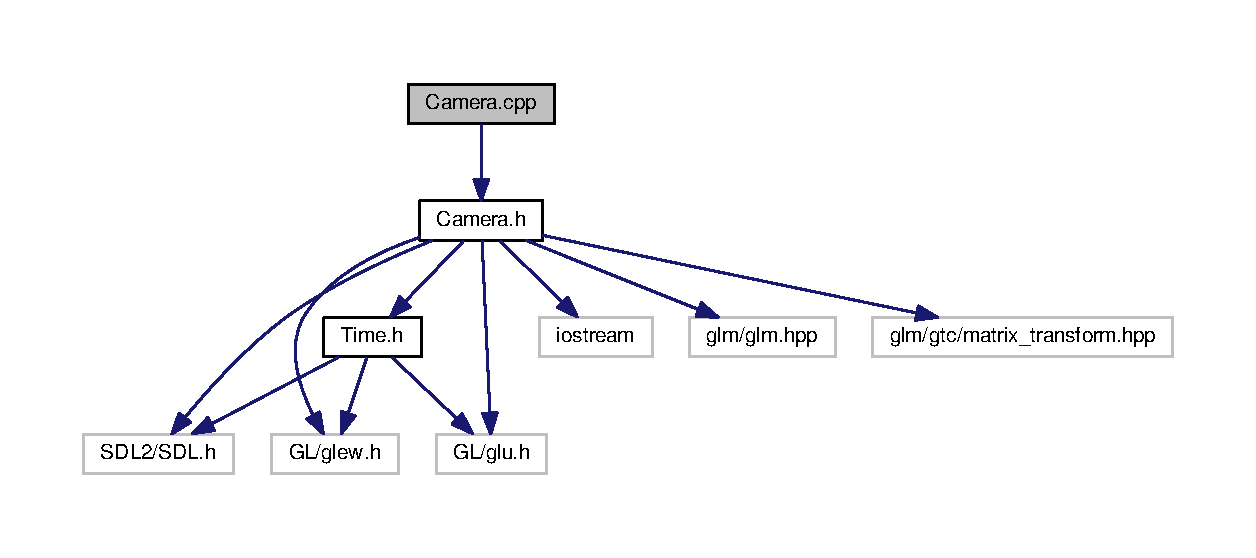
\includegraphics[width=350pt]{_camera_8cpp__incl}
\end{center}
\end{figure}

\hypertarget{_camera_8h}{}\section{Camera.\+h File Reference}
\label{_camera_8h}\index{Camera.\+h@{Camera.\+h}}
{\ttfamily \#include \char`\"{}S\+D\+L2/\+S\+D\+L.\+h\char`\"{}}\\*
{\ttfamily \#include \char`\"{}G\+L/glew.\+h\char`\"{}}\\*
{\ttfamily \#include \char`\"{}G\+L/glu.\+h\char`\"{}}\\*
{\ttfamily \#include \char`\"{}Time.\+h\char`\"{}}\\*
{\ttfamily \#include $<$iostream$>$}\\*
{\ttfamily \#include \char`\"{}glm/glm.\+hpp\char`\"{}}\\*
{\ttfamily \#include \char`\"{}glm/gtc/matrix\+\_\+transform.\+hpp\char`\"{}}\\*
Include dependency graph for Camera.\+h\+:\nopagebreak
\begin{figure}[H]
\begin{center}
\leavevmode
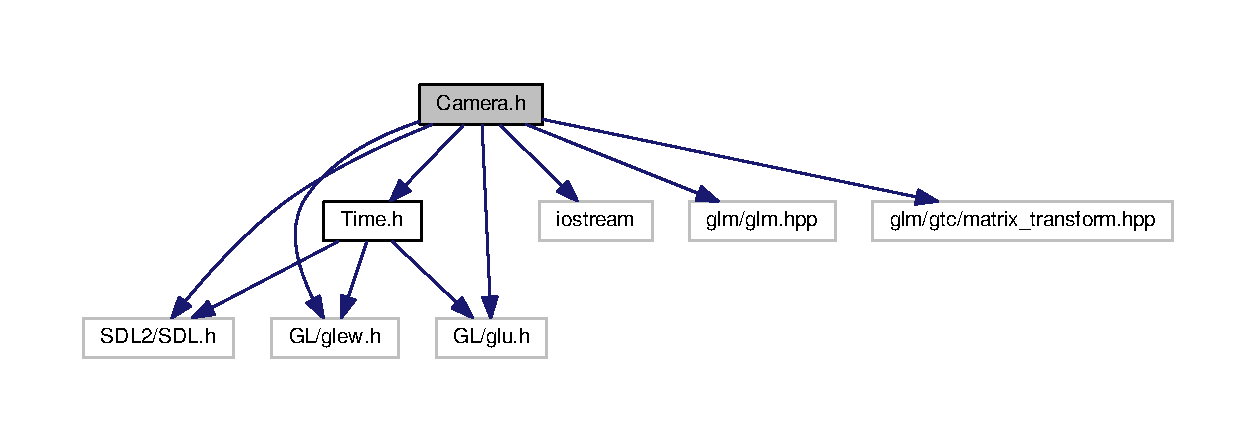
\includegraphics[width=350pt]{_camera_8h__incl}
\end{center}
\end{figure}
This graph shows which files directly or indirectly include this file\+:\nopagebreak
\begin{figure}[H]
\begin{center}
\leavevmode
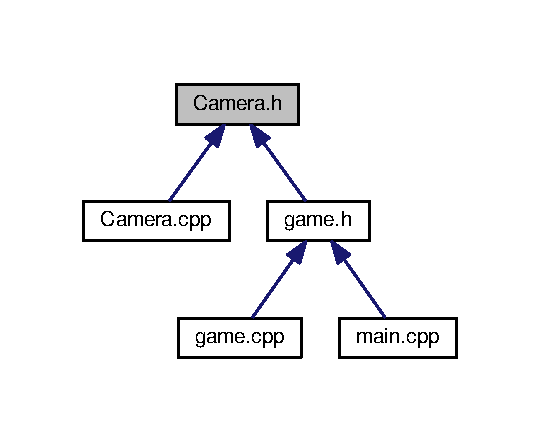
\includegraphics[width=259pt]{_camera_8h__dep__incl}
\end{center}
\end{figure}
\subsection*{Classes}
\begin{DoxyCompactItemize}
\item 
class \hyperlink{class_camera}{Camera}
\end{DoxyCompactItemize}
\subsection*{Macros}
\begin{DoxyCompactItemize}
\item 
\#define \hyperlink{_camera_8h_a816ab7d5c2ce1f0a01216042837beb93}{G\+L\+M\+\_\+\+F\+O\+R\+C\+E\+\_\+\+R\+A\+D\+I\+A\+N\+S}
\end{DoxyCompactItemize}


\subsection{Macro Definition Documentation}
\hypertarget{_camera_8h_a816ab7d5c2ce1f0a01216042837beb93}{}\index{Camera.\+h@{Camera.\+h}!G\+L\+M\+\_\+\+F\+O\+R\+C\+E\+\_\+\+R\+A\+D\+I\+A\+N\+S@{G\+L\+M\+\_\+\+F\+O\+R\+C\+E\+\_\+\+R\+A\+D\+I\+A\+N\+S}}
\index{G\+L\+M\+\_\+\+F\+O\+R\+C\+E\+\_\+\+R\+A\+D\+I\+A\+N\+S@{G\+L\+M\+\_\+\+F\+O\+R\+C\+E\+\_\+\+R\+A\+D\+I\+A\+N\+S}!Camera.\+h@{Camera.\+h}}
\subsubsection[{G\+L\+M\+\_\+\+F\+O\+R\+C\+E\+\_\+\+R\+A\+D\+I\+A\+N\+S}]{\setlength{\rightskip}{0pt plus 5cm}\#define G\+L\+M\+\_\+\+F\+O\+R\+C\+E\+\_\+\+R\+A\+D\+I\+A\+N\+S}\label{_camera_8h_a816ab7d5c2ce1f0a01216042837beb93}
Basic camera class.\+object created and used from within \hyperlink{class_game_aeae97cec35573c668d3f222a58f53255}{Game\+::gameloop} 

Definition at line 13 of file Camera.\+h.


\hypertarget{game_8cpp}{}\section{game.\+cpp File Reference}
\label{game_8cpp}\index{game.\+cpp@{game.\+cpp}}
{\ttfamily \#include \char`\"{}game.\+h\char`\"{}}\\*
Include dependency graph for game.\+cpp\+:\nopagebreak
\begin{figure}[H]
\begin{center}
\leavevmode
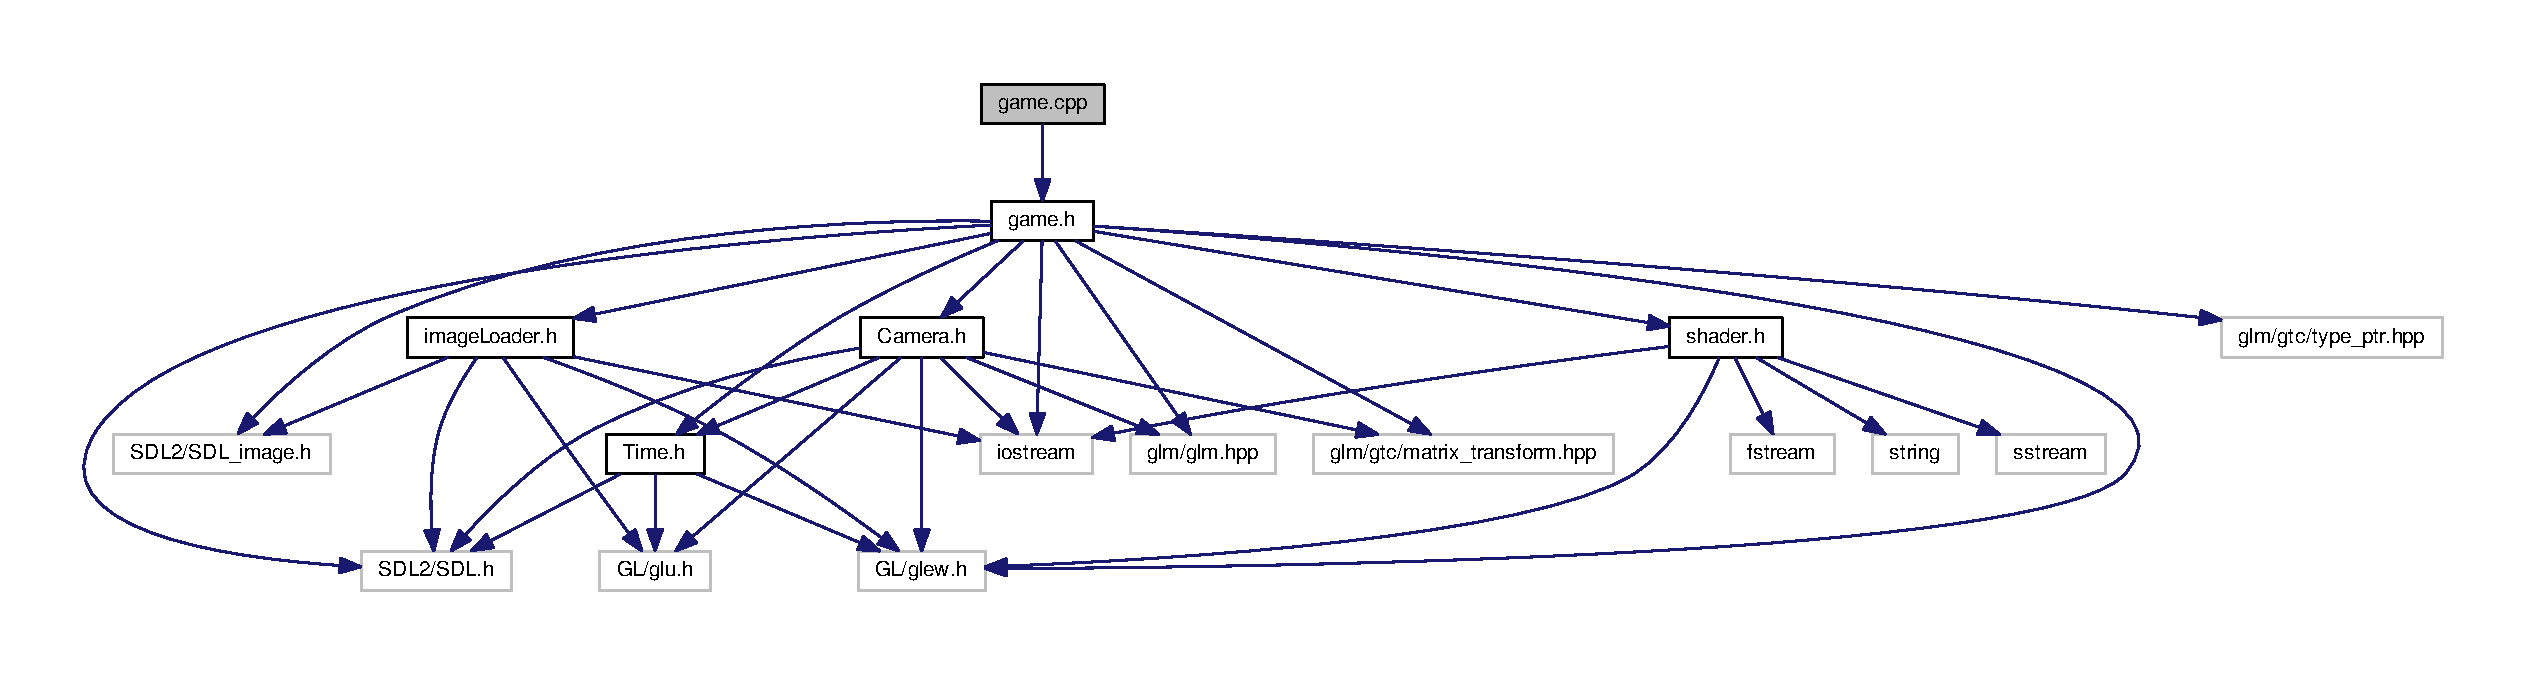
\includegraphics[width=350pt]{game_8cpp__incl}
\end{center}
\end{figure}

\hypertarget{game_8h}{}\section{game.\+h File Reference}
\label{game_8h}\index{game.\+h@{game.\+h}}
{\ttfamily \#include \char`\"{}S\+D\+L2/\+S\+D\+L.\+h\char`\"{}}\\*
{\ttfamily \#include \char`\"{}S\+D\+L2/\+S\+D\+L\+\_\+image.\+h\char`\"{}}\\*
{\ttfamily \#include \char`\"{}G\+L/glew.\+h\char`\"{}}\\*
{\ttfamily \#include $<$iostream$>$}\\*
{\ttfamily \#include \char`\"{}shader.\+h\char`\"{}}\\*
{\ttfamily \#include \char`\"{}image\+Loader.\+h\char`\"{}}\\*
{\ttfamily \#include \char`\"{}Camera.\+h\char`\"{}}\\*
{\ttfamily \#include \char`\"{}Time.\+h\char`\"{}}\\*
{\ttfamily \#include \char`\"{}glm/glm.\+hpp\char`\"{}}\\*
{\ttfamily \#include $<$glm/gtc/matrix\+\_\+transform.\+hpp$>$}\\*
{\ttfamily \#include $<$glm/gtc/type\+\_\+ptr.\+hpp$>$}\\*
Include dependency graph for game.\+h\+:\nopagebreak
\begin{figure}[H]
\begin{center}
\leavevmode
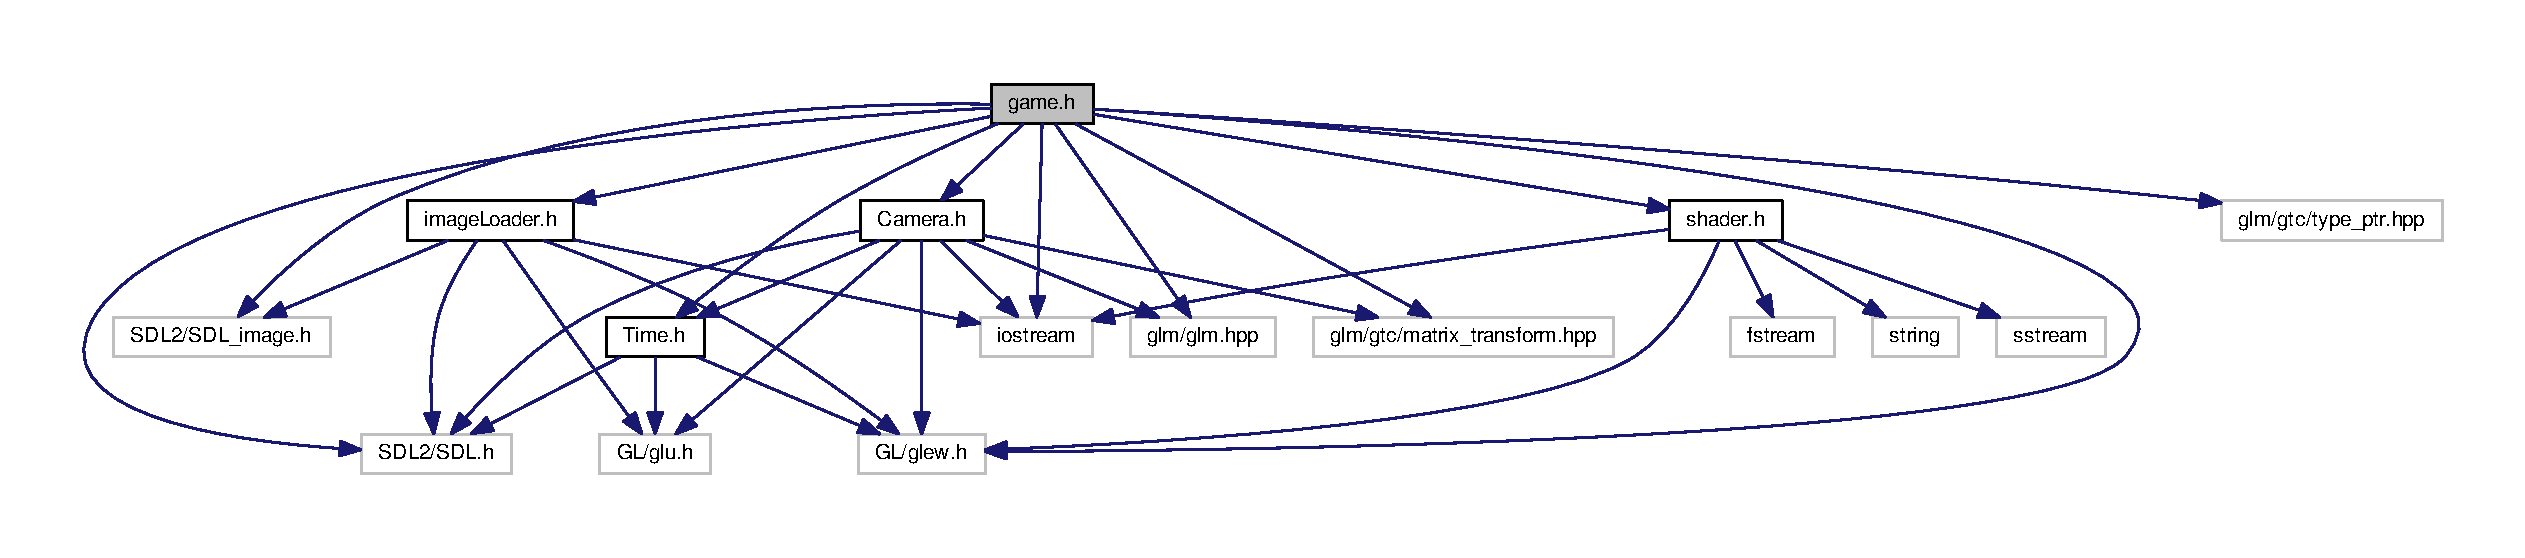
\includegraphics[width=350pt]{game_8h__incl}
\end{center}
\end{figure}
This graph shows which files directly or indirectly include this file\+:\nopagebreak
\begin{figure}[H]
\begin{center}
\leavevmode
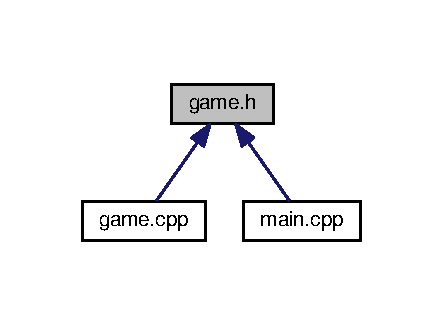
\includegraphics[width=213pt]{game_8h__dep__incl}
\end{center}
\end{figure}
\subsection*{Classes}
\begin{DoxyCompactItemize}
\item 
class \hyperlink{class_game}{Game}
\end{DoxyCompactItemize}
\subsection*{Macros}
\begin{DoxyCompactItemize}
\item 
\#define \hyperlink{game_8h_a816ab7d5c2ce1f0a01216042837beb93}{G\+L\+M\+\_\+\+F\+O\+R\+C\+E\+\_\+\+R\+A\+D\+I\+A\+N\+S}
\end{DoxyCompactItemize}


\subsection{Macro Definition Documentation}
\hypertarget{game_8h_a816ab7d5c2ce1f0a01216042837beb93}{}\index{game.\+h@{game.\+h}!G\+L\+M\+\_\+\+F\+O\+R\+C\+E\+\_\+\+R\+A\+D\+I\+A\+N\+S@{G\+L\+M\+\_\+\+F\+O\+R\+C\+E\+\_\+\+R\+A\+D\+I\+A\+N\+S}}
\index{G\+L\+M\+\_\+\+F\+O\+R\+C\+E\+\_\+\+R\+A\+D\+I\+A\+N\+S@{G\+L\+M\+\_\+\+F\+O\+R\+C\+E\+\_\+\+R\+A\+D\+I\+A\+N\+S}!game.\+h@{game.\+h}}
\subsubsection[{G\+L\+M\+\_\+\+F\+O\+R\+C\+E\+\_\+\+R\+A\+D\+I\+A\+N\+S}]{\setlength{\rightskip}{0pt plus 5cm}\#define G\+L\+M\+\_\+\+F\+O\+R\+C\+E\+\_\+\+R\+A\+D\+I\+A\+N\+S}\label{game_8h_a816ab7d5c2ce1f0a01216042837beb93}
Class to initialise S\+D\+L and open\+G\+L also contains the main loop and render functions. object is created and used from \hyperlink{main_8cpp}{main.\+cpp} 

Definition at line 19 of file game.\+h.


\hypertarget{image_loader_8cpp}{}\section{image\+Loader.\+cpp File Reference}
\label{image_loader_8cpp}\index{image\+Loader.\+cpp@{image\+Loader.\+cpp}}
{\ttfamily \#include \char`\"{}image\+Loader.\+h\char`\"{}}\\*
Include dependency graph for image\+Loader.\+cpp\+:\nopagebreak
\begin{figure}[H]
\begin{center}
\leavevmode
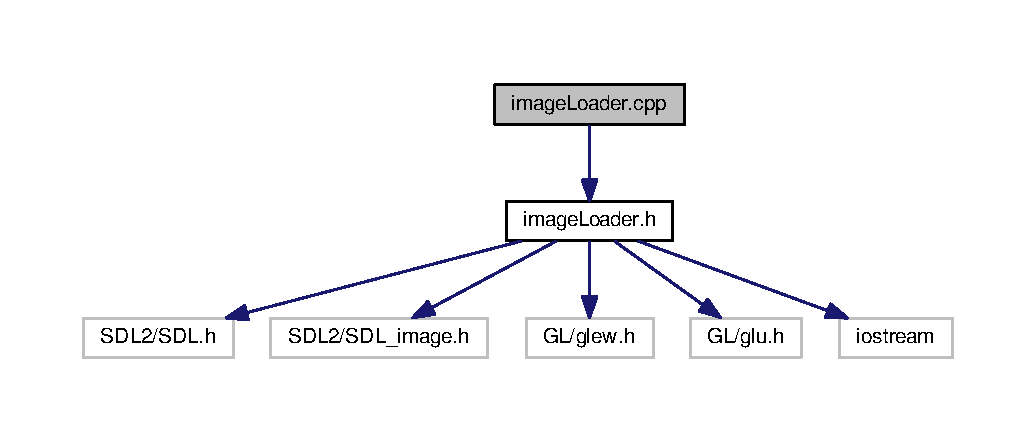
\includegraphics[width=350pt]{image_loader_8cpp__incl}
\end{center}
\end{figure}

\hypertarget{image_loader_8h}{}\section{image\+Loader.\+h File Reference}
\label{image_loader_8h}\index{image\+Loader.\+h@{image\+Loader.\+h}}
{\ttfamily \#include \char`\"{}S\+D\+L2/\+S\+D\+L.\+h\char`\"{}}\\*
{\ttfamily \#include \char`\"{}S\+D\+L2/\+S\+D\+L\+\_\+image.\+h\char`\"{}}\\*
{\ttfamily \#include \char`\"{}G\+L/glew.\+h\char`\"{}}\\*
{\ttfamily \#include \char`\"{}G\+L/glu.\+h\char`\"{}}\\*
{\ttfamily \#include $<$iostream$>$}\\*
Include dependency graph for image\+Loader.\+h\+:\nopagebreak
\begin{figure}[H]
\begin{center}
\leavevmode
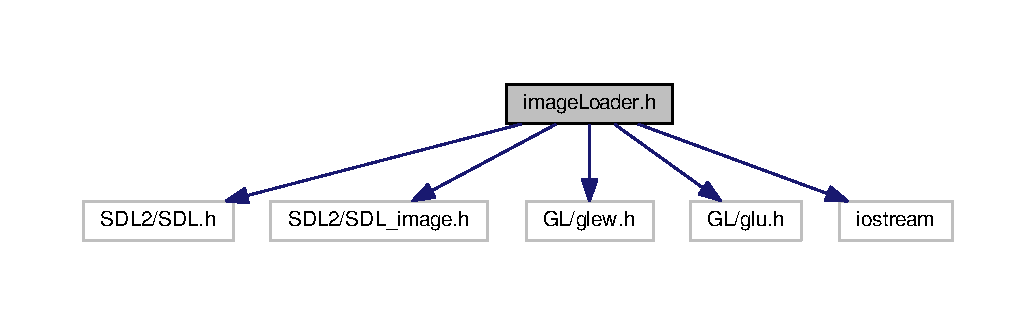
\includegraphics[width=350pt]{image_loader_8h__incl}
\end{center}
\end{figure}
This graph shows which files directly or indirectly include this file\+:\nopagebreak
\begin{figure}[H]
\begin{center}
\leavevmode
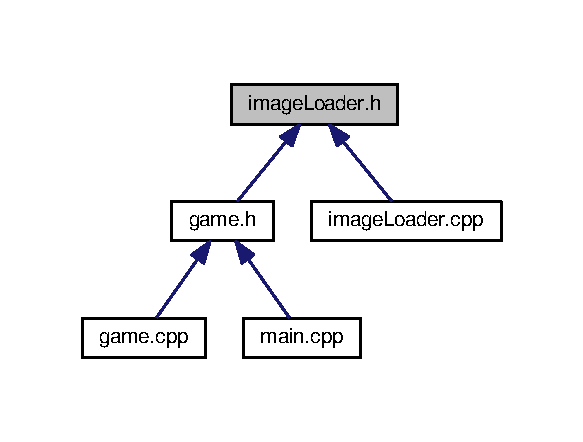
\includegraphics[width=280pt]{image_loader_8h__dep__incl}
\end{center}
\end{figure}
\subsection*{Classes}
\begin{DoxyCompactItemize}
\item 
class \hyperlink{classimage_loader}{image\+Loader}
\end{DoxyCompactItemize}

\hypertarget{main_8cpp}{}\section{main.\+cpp File Reference}
\label{main_8cpp}\index{main.\+cpp@{main.\+cpp}}
{\ttfamily \#include \char`\"{}game.\+h\char`\"{}}\\*
Include dependency graph for main.\+cpp\+:\nopagebreak
\begin{figure}[H]
\begin{center}
\leavevmode
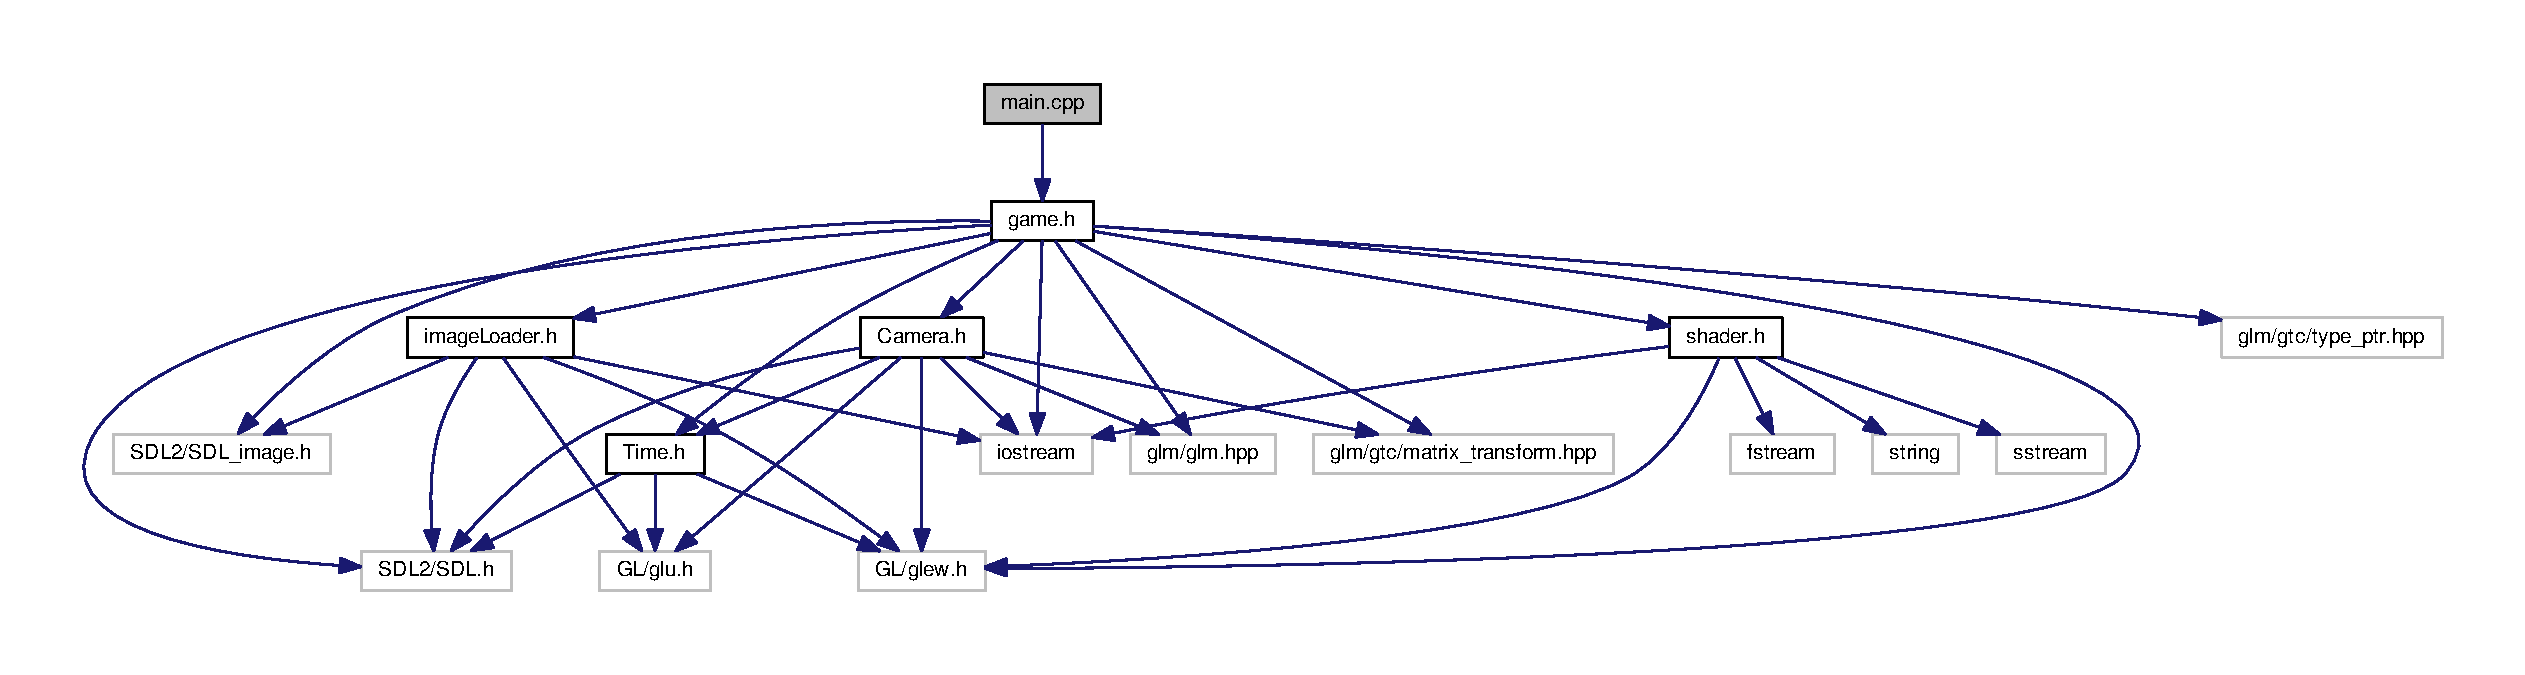
\includegraphics[width=350pt]{main_8cpp__incl}
\end{center}
\end{figure}
\subsection*{Functions}
\begin{DoxyCompactItemize}
\item 
int \hyperlink{main_8cpp_ae66f6b31b5ad750f1fe042a706a4e3d4}{main} ()
\end{DoxyCompactItemize}
\subsection*{Variables}
\begin{DoxyCompactItemize}
\item 
\hyperlink{class_game}{Game} $\ast$ \hyperlink{main_8cpp_a58bdb5643d0814ac4e697a1564b79b70}{game} = new \hyperlink{class_game}{Game}()
\end{DoxyCompactItemize}


\subsection{Function Documentation}
\hypertarget{main_8cpp_ae66f6b31b5ad750f1fe042a706a4e3d4}{}\index{main.\+cpp@{main.\+cpp}!main@{main}}
\index{main@{main}!main.\+cpp@{main.\+cpp}}
\subsubsection[{main}]{\setlength{\rightskip}{0pt plus 5cm}int main (
\begin{DoxyParamCaption}
{}
\end{DoxyParamCaption}
)}\label{main_8cpp_ae66f6b31b5ad750f1fe042a706a4e3d4}
Main entry point.

Definition at line 5 of file main.\+cpp.



Here is the call graph for this function\+:\nopagebreak
\begin{figure}[H]
\begin{center}
\leavevmode
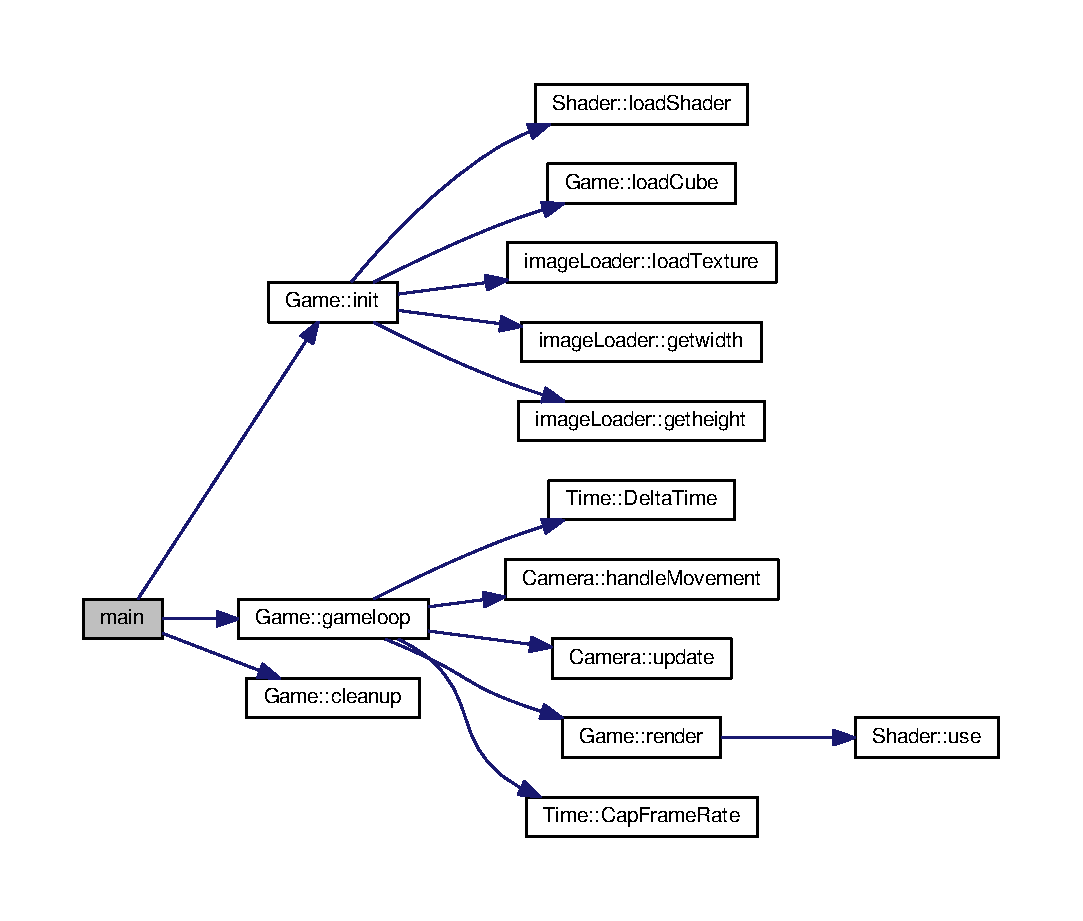
\includegraphics[width=350pt]{main_8cpp_ae66f6b31b5ad750f1fe042a706a4e3d4_cgraph}
\end{center}
\end{figure}




\subsection{Variable Documentation}
\hypertarget{main_8cpp_a58bdb5643d0814ac4e697a1564b79b70}{}\index{main.\+cpp@{main.\+cpp}!game@{game}}
\index{game@{game}!main.\+cpp@{main.\+cpp}}
\subsubsection[{game}]{\setlength{\rightskip}{0pt plus 5cm}{\bf Game}$\ast$ game = new {\bf Game}()}\label{main_8cpp_a58bdb5643d0814ac4e697a1564b79b70}


Definition at line 3 of file main.\+cpp.


\hypertarget{shader_8cpp}{}\section{shader.\+cpp File Reference}
\label{shader_8cpp}\index{shader.\+cpp@{shader.\+cpp}}
{\ttfamily \#include \char`\"{}shader.\+h\char`\"{}}\\*
{\ttfamily \#include $<$fstream$>$}\\*
{\ttfamily \#include $<$string$>$}\\*
{\ttfamily \#include $<$sstream$>$}\\*
{\ttfamily \#include $<$iostream$>$}\\*
Include dependency graph for shader.\+cpp\+:\nopagebreak
\begin{figure}[H]
\begin{center}
\leavevmode
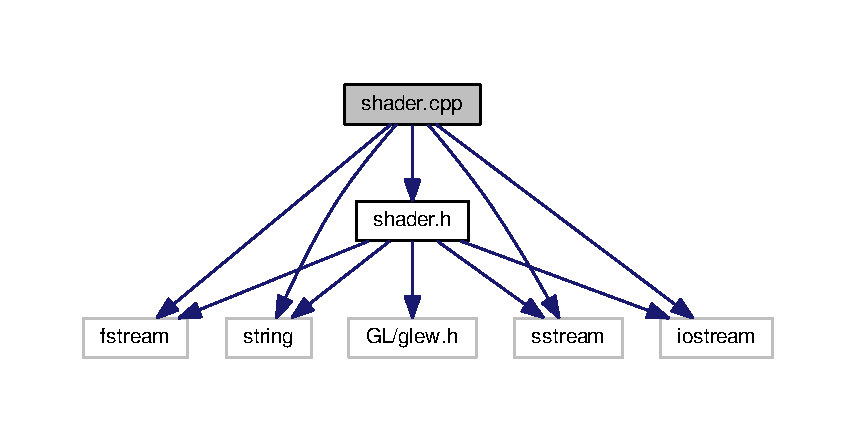
\includegraphics[width=350pt]{shader_8cpp__incl}
\end{center}
\end{figure}

\hypertarget{shader_8h}{}\section{shader.\+h File Reference}
\label{shader_8h}\index{shader.\+h@{shader.\+h}}
{\ttfamily \#include $<$fstream$>$}\\*
{\ttfamily \#include $<$string$>$}\\*
{\ttfamily \#include $<$sstream$>$}\\*
{\ttfamily \#include $<$iostream$>$}\\*
{\ttfamily \#include \char`\"{}G\+L/glew.\+h\char`\"{}}\\*
Include dependency graph for shader.\+h\+:\nopagebreak
\begin{figure}[H]
\begin{center}
\leavevmode
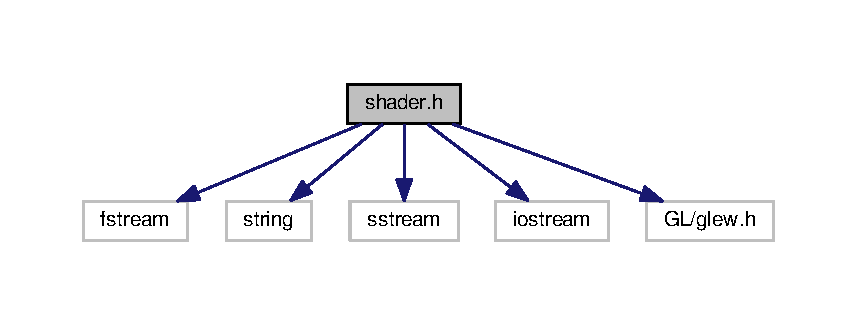
\includegraphics[width=350pt]{shader_8h__incl}
\end{center}
\end{figure}
This graph shows which files directly or indirectly include this file\+:\nopagebreak
\begin{figure}[H]
\begin{center}
\leavevmode
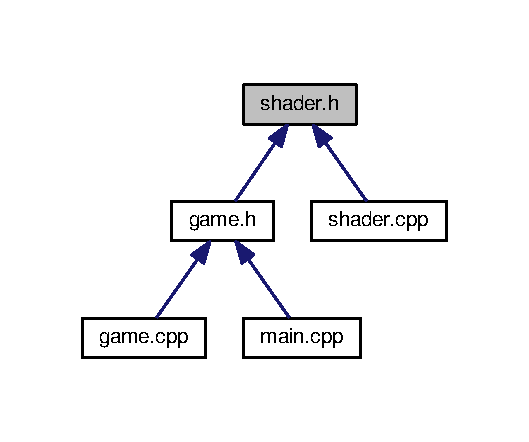
\includegraphics[width=254pt]{shader_8h__dep__incl}
\end{center}
\end{figure}
\subsection*{Classes}
\begin{DoxyCompactItemize}
\item 
class \hyperlink{class_shader}{Shader}
\end{DoxyCompactItemize}

\hypertarget{_time_8cpp}{}\section{Time.\+cpp File Reference}
\label{_time_8cpp}\index{Time.\+cpp@{Time.\+cpp}}
{\ttfamily \#include \char`\"{}Time.\+h\char`\"{}}\\*
Include dependency graph for Time.\+cpp\+:\nopagebreak
\begin{figure}[H]
\begin{center}
\leavevmode
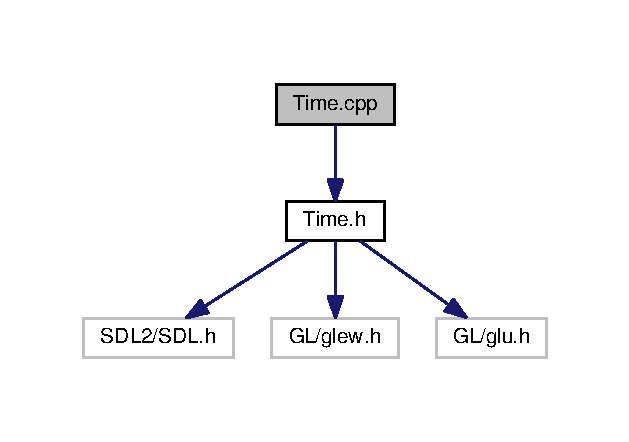
\includegraphics[width=302pt]{_time_8cpp__incl}
\end{center}
\end{figure}

\hypertarget{_time_8h}{}\section{Time.\+h File Reference}
\label{_time_8h}\index{Time.\+h@{Time.\+h}}
{\ttfamily \#include \char`\"{}S\+D\+L2/\+S\+D\+L.\+h\char`\"{}}\\*
{\ttfamily \#include \char`\"{}G\+L/glew.\+h\char`\"{}}\\*
{\ttfamily \#include \char`\"{}G\+L/glu.\+h\char`\"{}}\\*
Include dependency graph for Time.\+h\+:\nopagebreak
\begin{figure}[H]
\begin{center}
\leavevmode
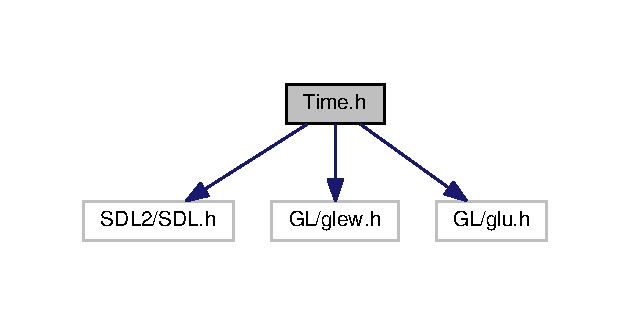
\includegraphics[width=302pt]{_time_8h__incl}
\end{center}
\end{figure}
This graph shows which files directly or indirectly include this file\+:\nopagebreak
\begin{figure}[H]
\begin{center}
\leavevmode
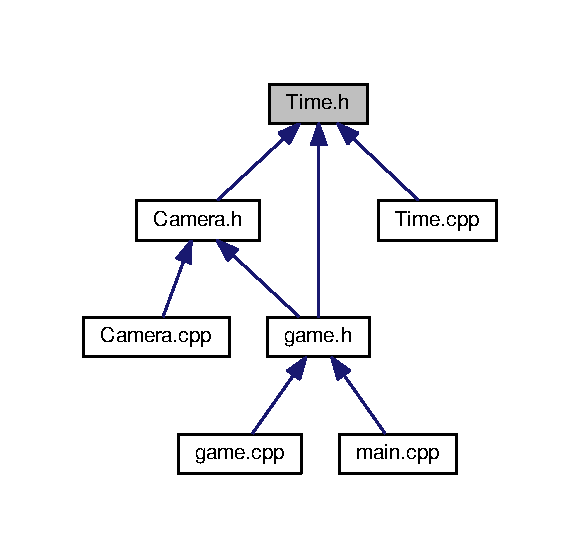
\includegraphics[width=278pt]{_time_8h__dep__incl}
\end{center}
\end{figure}
\subsection*{Classes}
\begin{DoxyCompactItemize}
\item 
class \hyperlink{class_time}{Time}
\end{DoxyCompactItemize}

%--- End generated contents ---

% Index
\backmatter
\newpage
\phantomsection
\clearemptydoublepage
\addcontentsline{toc}{chapter}{Index}
\printindex

\end{document}
